\documentclass[11pt,titlepage,uplatex]{ujreport}
% 他のパッケージ・スタイルを使う場合には適宜追加
\usepackage{cisbmdstyle}
\usepackage{indentfirst}
\usepackage{url}
\usepackage[dvipdfmx]{graphicx}
% 新しい定義を使う場合には適宜追加
\renewcommand{\bibname}{参考文献}
\usepackage[deluxe]{otf}

% ハイパーリンクを有効にする
\usepackage[dvipdfmx]{hyperref}
\usepackage{pxjahyper}
\hypersetup{
 setpagesize=false,
 bookmarksnumbered=true,%
 bookmarksopen=true,%
 colorlinks=true,%
 linkcolor=black,
 citecolor=black,
 urlcolor=black,
}

%%
%% 主に表紙を作成するための情報
%%

%%  タイトル
\title{スタイルファイルを用いた\\
       \LaTeX による卒業・修士・博士論文の作成}
%%  英語タイトル
%\etitle{Compiling Bachelor's/Master's/Doctor's Thesis based on \TeX\\
%       using Our Style Files at Doshisha University}

% 要旨
%   (行の先頭が ``\\'' で始まらないようにすること)
% 修士論文の場合は 1,000 〜 2,000 字程度で記載すること.
\abstract{
これで41字$\times$37行.
文字カウントをするため,章毎の改ページが行われるようになっている.
編集のしかたについては,\texttt{sample\_latex.tex} 内部のコメントや付録を参
考のこと.

なお,卒業論文の場合は 1,000 字程度,修士,博士論文の場合は 1,000 〜 2,000 字
程度で記載すること.
}

%% 英文要旨
%\eabstract{
%This is abstract.
%}

%%  著者名
\author{文情 太郎}

%%  担当教員 (卒業論文)
%%    (姓と名,名と称号の間に半角スペースを入れる)
%%
%% 4 名まで記入可能.4 名以下の場合は {}{} を利用.
%% 2 名
%\advisers{主担当教員}{新島 襄 教授}
%         {副担当教員}{新島 八重 教授}
%         {}{}
%         {}{}
%% 3 名
%\advisers{主担当教員}{新島 襄 教授}
%         {副担当教員}{新島 八重 教授}
%         {副担当教員}{ドウェイト・ウィットニー・ラーネッド 教授}
%         {}{}
\advisers{主担当教員}{新島 襄 教授}
         {副担当教員}{新島 八重 教授}
         {副担当教員}{ドウェイト・ウィットニー・ラーネッド 教授}
         {副担当教員}{ジェローム・デイヴィス 教授}

%%  担当教員 (修士,博士論文)
%%    (姓と名,名と称号の間に半角スペースを入れる)
%%
%% 最大 3 名まで記入可能.
%% 空白 {}{} は削除不可
%\supervisers{}{}
%            {}{}
%            {指導教員}{村上 征勝 教授}
%\supervisers{}{}
%            {指導教員}{村上 征勝 教授}
%            {指導教員}{金 明哲 教授}
%\supervisers{主査}{村上 征勝 教授}
%            {副査}{金 明哲 教授}
%            {副査}{川崎 廣吉 教授}


%%  卒業論文・修士論文・博士論文 (以下のいずれかを選択)
\course{bachelor}	% 卒業論文
%\course{master}  	% 修士論文
%\course{doctor}  	% 博士論文

%%  学科・課程
\department{文化情報}                            % 学部
%\department{文化情報学専攻 博士課程 (前期課程)}  % 修士
%\department{文化情報学専攻 博士課程 (後期課程)}  % 博士

%%  学籍番号
\studentid{1108XX0000}
%\studentid{38100100}

%%  入学年度 (卒業論文のみ)
\eyear{20XX}

%%  卒業年度
\gyear{20XX}

%%  論文提出日 (卒業,修士論文のみ)
\date{20XX年12月}
%\西暦		
% \dateを指定せずに\西暦を有効にしておくと,コンパイル
% した日付が提出日として自動的に設定される.

%%%%%%%%%%%%%%%%%%%%%%%%%%%%%%%%%%%%%%%%%%%%%%%%%%%%%%%%%%%%%%%%%%%%%%%%
\begin{document}
% 表紙
%\makecover
% 中表紙
\makeicover
% 写真ページ (修士・博士論文のみ)
%\makepcover
% 要旨ページ (卒業論文) / 概要ページ (修士・博士論文)
\abstractpage
%%  目次
\tableofcontents
%  図目次 (図目次をいれたければ以下のコメントをはずす)
%\listoffigures
%  表目次 (表目次をいれたければ以下のコメントをはずす)
%\listoftables

\newpage
\pagenumbering{arabic}	% 以降のページ番号を算用数字に

%%%%%%%%%%%%%%%%%%%%%%%%%%%%%%%%%%%%%%%%%%%%%%%%%%%%%%%%%%%%%%%%%%%%%%%%

%%
%%  本文はここから
%%
\chapter{はじめに}
食事というものは我々の生活にとても密着しているものであり,日々の健康を支
えるためには欠かせないものである.
効率の良い栄養摂取方法を考慮したレシピや,彩り豊かなレシピとして,様々な
食材を使ったレシピが数多く考案され,料理本として出版されたり,Webに公開
されたりしている.
その中でも,Webで公開されているレシピの数は膨大にある.
代表的なレシピ検索サイトであるクックパッド\footnote{クックパッド
(\url{http://cookpad.com/})2010年12月現在}では, 900, 845品ものレシピ
が公開されている上,ユーザの投稿によって日々増え続けている.
また,検索サイトだけではなく,キューピー3分クッキング\footnote{キューピー
3分クッキング(\url{http://www.ntv.co.jp/3min/index.html})}
といった毎日のレシピ公開サイトや,個人のブログでも数多くのレシピが公開さ
れている.
しかし,それら一つ一つのサイトの中には膨大なレシピが公開されており,その
中からユーザ自身に適合するレシピを探し出すことは困難である.

また,健康的な生活を送るためには日々の食生活管理が重要である.現代の日本
では糖尿病や肥満,心臓病といった生活習慣病が問題になっている.
平成20年の国民健康・栄養調査\footnote{国民健康・栄養調査
(\url{http://www.mhlw.go.jp/houdou/2008/04/h0430-2.html})}
によると糖尿病が強く疑われる人は約820万人,糖尿病の可能性が否定できない
人は約1,050万人であり,高血圧症有病者は約3,970万人,正常高値血圧者や約
1,520万人と推定される.
また,メタボリックシンドロームが強く疑われる人の割合は男性25.3%,女性
10.6%であり,メタボリックシンドロームの予備群と考えられる人の割合は男性
21.9%,女性8.3%である.
このことから,男性の場合約半数がメタボリックシンドロームかその予備群とい
う結果となっている.
厚生労働省,農林水産省,文部科学省では,これらのような生活習慣病の予防に
効果的であり,身近なものとして正しい食生活を送ることを推進している.その
ために国民ひとりひとりが食生活改善に取り組むよう,「食生活指針」
\footnote{食生活指針
(\url{http://www1.mhlw.go.jp/houdou/1203/h0323-1\_11.html})}を策定している.

しかしながら,栄養素バランスが整った食生活は必ずしも多くの人に意識され,
実践されているとはいえない状態である.
昨今の日本は飽食の時代といわれるほどに食生活は豊かになったが,スナック菓
子や清涼飲料水の取りすぎなどにより,体調を崩す人が出てきている.また,朝
食を食べない人が年々増加しているという現状もある \cite{jikkyo10}.

このような問題を食生活の面から改善し,健康に生きるためには栄養素バランス
を考慮した献立がとても重要である.
しかしながら,現状において人々が生活の中でバランスの良い献立を考えるため
には専門的な知識と膨大なレシピの中から適合するものを選出する労力が必要で
ある.
そのため,正確に栄養素バランスが整った献立を考え,日々の食生活に反映する
事は困難である.

そこで本研究では,個人の年齢や性別,体調,欲求などから各人に適応する栄養
素バランスを制定し,それに合わせた献立を推薦する手法を提案する.
本手法により,専門的な知識を必要とせず,個人の体調や欲求に合わせた献立を
簡単に作成することが可能となる.

\chapter{関連研究}
本章では関連研究として,情報推薦技術について述べた後,栄養素バランスを考
慮したレシピ推薦に関する研究について述べ,それらを踏まえて本研究の目標に
ついて述べる.

\section{情報推薦技術}
情報推薦システムにおいて,ユーザに適した情報を抽出し,推薦するためにコン
テンツフィルタリング(Content-based filtering)と,協調フィルタリング
( Collaborative filtering)という二つのフィルタリング技術を利用している
\cite{hijikata04}.

コンテンツフィルタリングは,推薦する情報の内容に基づき,情報の取捨選択を
行うものである.具体的にはアイテムに付与されているコンテンツ情報から,ユー
ザが必要としている情報と同じコンテンツ情報を持ったアイテムを推薦する.
例えば,ユーザが本を買う際に,すべての本情報から「アドベンチャー」や「恋
愛小説」といったジャンルというコンテンツ情報を元にユーザがほしい本を推薦
する.

協調フィルタリングは,コンテンツ情報は利用せずに,ネットワーク上に存在す
る同じ好みを持ったコミュニティを発見し,そのコミュニティが共通して好む情
報を選択するものである.
これはコンテンツ情報さえあれば新しいアイテム等も推薦可能ではあるが,コン
テンツ情報が付与されていないものは推薦されないため,正確な情報付与が必要
となる.
これは前提概念として,ある一つのアイテムに対して同じ評価をもつ者は別のア
イテムにおいても同様の評価をするだろうというものがある.
例えば,ユーザA,Bとアイテムa,b,c,dが存在し,ユーザAが購入したアイテムが
a,b,c,d,ユーザBが購入したアイテムがa,c,dだったとする.この時,ユーザAと
ユーザBは同じ3種類のアイテムを購入しているところから,ユーザAとユーザB
が同じ嗜好を持っているとみなすことができる.そこで,ユーザAは購入済みだ
がユーザBは未購入であるbを推薦する,というものである.
しかし,協調フィルタリングの場合,新しいアイテムが出てきた際や購入履歴の
ないアイテムがある場合,ユーザとのネットワークがつながらないため,他のユー
ザにも推薦されない,というゼロ頻度問題が懸念される.

\section{ユーザプロファイリング技術}
上記で挙げた情報のフィルタリング技術を用いて,膨大な情報の中から個人に適
した情報を選択し,個人に適した方法で表示することが重要である.
このようなサービスをパーソナライゼーションと呼ぶ.パーソナライゼーション
を行うためには,ユーザの興味や目的,おかれたコンテキストなどの情報を獲得
する必要がある.
この技術をユーザプロファイリング技術と呼ぶ.このユーザプロファイリング技
術には,大きく分けると明示的手法(explicit method)と暗黙的手法
(implicit method)の二種類が存在する \cite{hijikata04}.

明示的手法は,ユーザから直接に,興味に関する情報を入力してもらう方法であ
る.大きくは,ユーザの興味に関してトピックやキーワードの形でアンケートに
答えさせる方法,または閲覧したページにどれだけ興味があったかを数段階で評
価をすけさせる方法の2種類に分類できる.
この手法ではユーザが直接答えたものから興味にかんする情報を取得するため,
信頼性が高いという利点が挙げられる.
しかし,アンケートや閲覧後の評価はユーザに負担をかけるよいう問題点が挙げ
られる.

暗黙的手法は,ユーザのWeb閲覧時の挙動から,ユーザの興味に関する情報を取
得する方法である.
本手法には,閲覧したページのすべてにユーザが興味を持ったと仮定して,Web
ページのアクセス履歴を用いる方法と,何らかの方法でユーザが閲覧した情報に
興味の有無を推定する方法の2種類に分類できる.
後者の場合,興味の有無を推定するためにユーザが閲覧に費やした時間や,閲覧
中におけるマウス操作,閲覧中の視線などの方法がとられている.
この手法では,明示的手法のような興味に関する入力を強いないという利点が挙
げられる.
しかし,アクセス履歴や閲覧時間を用いる方法は,ページを表示させるという行
為だけで興味があると認識してしまうが,その行為でユーザの興味に関する情報
がすべて収集できるとは考えにくい.

\section{栄養素バランスを考慮した料理推薦に関する研究}
毎日の食生活を豊かにするためには栄養素バランスや摂取料理の種類の豊富さを
考慮し,献立を決定する必要がある.

苅米ら~\cite{karikome09}は最初に一つレシピを検索し,その出力された料理に
基づいて栄養素バランスの良い組み合わせを検索するというシステムを提案して
いる.
これは,オフライン処理とオンライン処理に分かれたシステムであり,オフライ
ン処理ではあらかじめweb からレシピを収集し,レシピから材料や様式などの情
報を抽出し,レシピのデータを作成する.
そして,食品群を対応付ける辞書を作成して食品群ごとに摂取量を計算する.
オンライン処理では,検索システムに検索条件を入力し,条件に合致するレシピ
をデータベースから検索する.
さらに,検索された料理に基づいて別の料理との関連度を計算し献立検索を行う.
これはユーザの年齢・性別より一般的に必要とされる栄養素を計算し,充足率を
判断していくものである.

李ら~\cite{li09}は栄養素バランスと個人の嗜好も考慮した料理推薦システムを
提案している.
これは,嗜好を考慮したレシピスコアと栄養素バランスを考慮したレシピスコア
の得点を足し合わせる事で栄養と嗜好との間にバランスが取れた料理推薦を可能
としている.
具体的には,レシピ中の推薦食材に含まれる不足栄養素の摂取量から計算した栄
養素バランスに関する得点と食事履歴から上田ら~\cite{ueda08}が提案した
TF-IDF(Term Frequency - Inverted Document Frequency)における単語の出現
頻度に基づき尺度化する考えを,食材の利用頻度の尺度化に応用した食材利用尺
度FF-IRF(Foodstuff Frequency - Inverted Recipe Frequency)を用いて計算
した嗜好に関する得点をに基づいて推薦スコアを算出している.
この手法のでは,個人の食材利用履歴を用いて個人の嗜好をレシピ検索に反映し
ているところが特徴である.


\section{本研究の目標}
2.3 節で挙げた料理検索では一般的に年齢と性別という観点から日本人に必要と
されている栄養素を基準にしている.
しかし,人は十人十色の生活を過ごしており,一様に同じ年齢・性別の人が同じ
栄養素を必要としているとは考えにくい.
個人に必要な栄養素を測るためには,体調や欲求といった個人の状況を考慮する必要がある.

そこで本研究では,栄養素バランスを考慮しながら,さらにユーザの体調や欲求
を把握することでよりそのユーザに必要な栄養素バランスを満たす献立を提案す
る.

\chapter{提案手法}
本研究では,先行研究にあるような従来の栄養素バランスを考慮した献立検索に加え,
ユーザの体調や欲求といった個人の状況を考慮した献立を推薦する手法を提案する.
これにより,ユーザの欲求や体調を自動的に献立推薦へ反映させる事が可能となる.
食材により栄養素バランスが整った献立推
薦や,その人の目的・欲求に合わせた料理を検索で
きるようにする.
\section{概要}
本研究で提案する献立推薦システムの構成を図\ref{システム図}に示す.
本システムではまず,各ユーザに適した目標栄養素バランスを設定し,朝食と昼
食に食べた料理で満たされた栄養素摂取量を差し引き,夕食に必要な栄養素バラ
ンスを算出する.
そして不足栄養素を補うよう主菜・副菜の順に推薦していき,夕食の献立を提案する.

一つの料理を選択した際に栄養素量が充足される割合(充足率)を算出し,より
充足率の高い料理を推薦ランキング上位に候補として推薦する.それを複数回繰
り返すことで充足率を向上させ,献立としてユーザに夕食を推薦する.
本システムでの献立推薦の流れを以下に示す.
\begin{figure}[tbh]
  \centering
%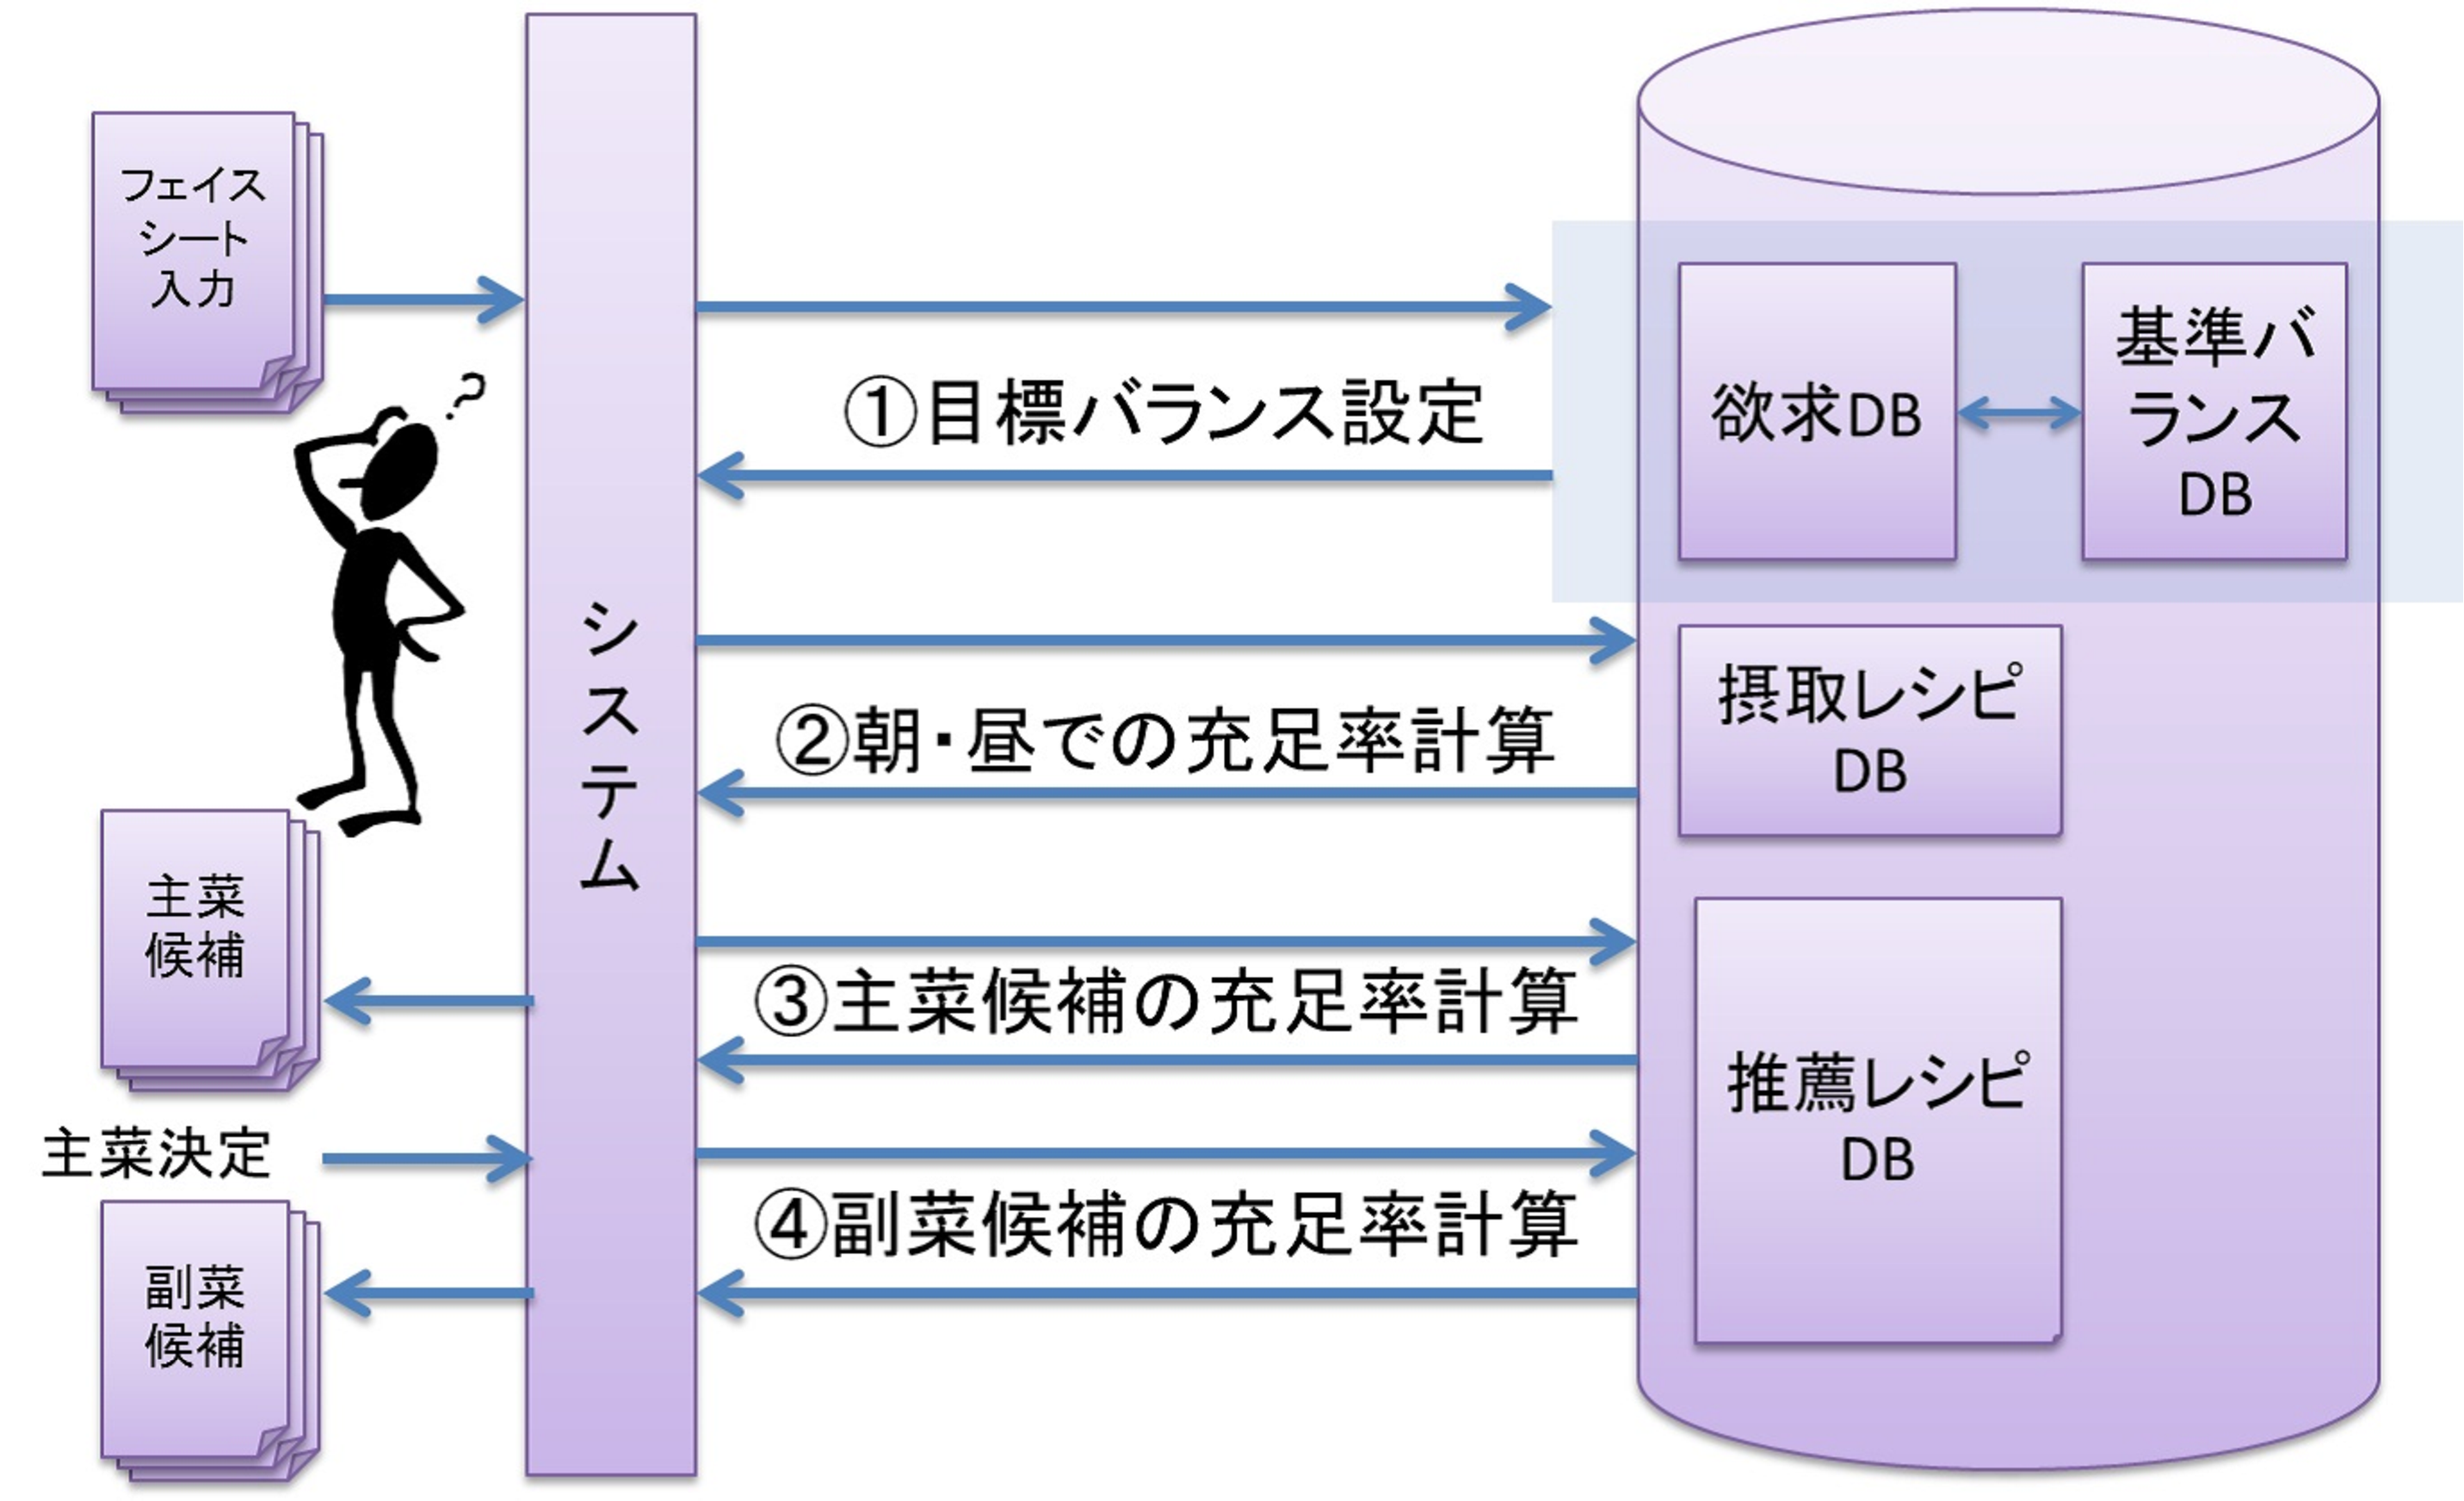
\includegraphics[scale=0.3,clip]{system.pdf}
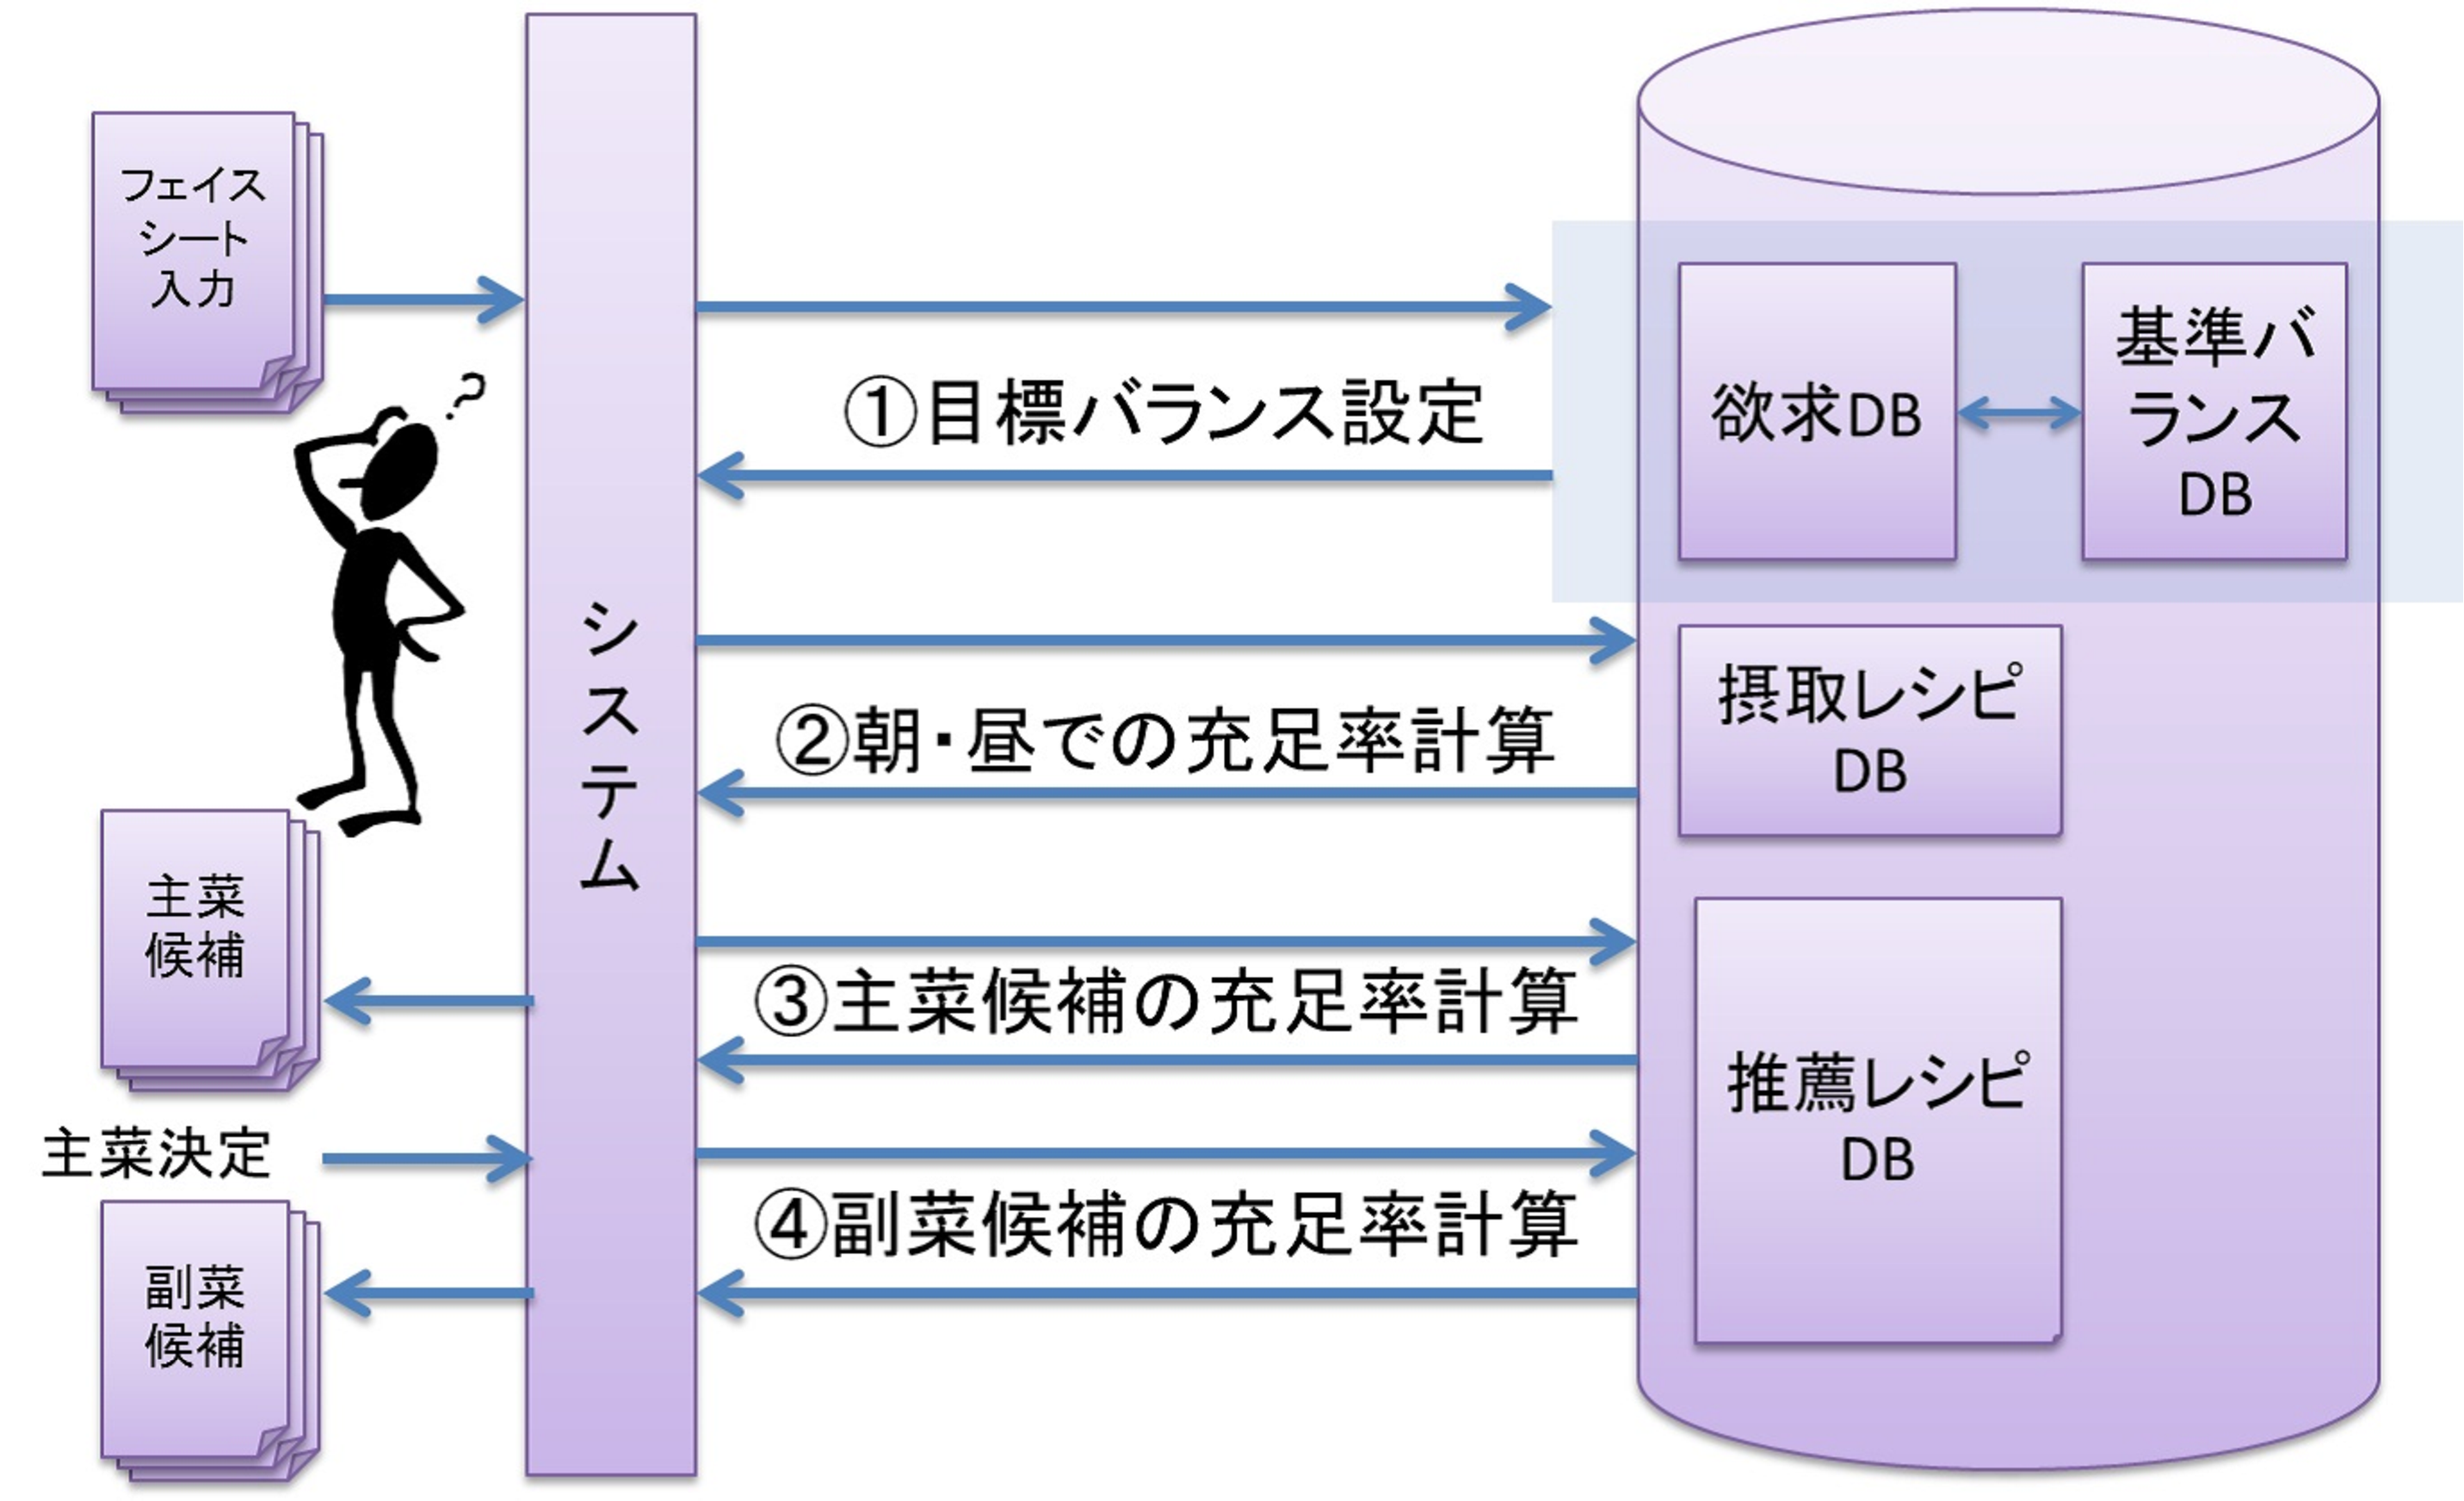
\includegraphics[scale=0.3]{system.pdf}
\caption{システム図}
\label{システム図}
\end{figure}
\begin{enumerate}
\item{目標バランスを設定}\\
     入力された年齢,性別から基準となる栄養素バランスを暫定的に決定し,
     欲求項目に設定され調整値と組み合わせて目標バランスを設定する.
\item{朝食,昼食での充足率計算}\\
     入力された朝食,昼食に食べた料理に一番近い献立から夕食を摂取する前
     の栄養素が目標栄養素量に充足されている割合(充足率)を算出し,今現
     在での各栄養素の摂取バランスを測定する.
\item{主菜候補の充足率計算}\\
     目標栄養素量から朝食,昼食に摂取した栄養素量を差し引いた上での夕食
     で摂取すべき必要栄養素量を算出し,それぞれの栄養素において過不足な
     いよう主菜を推薦する.
     この時,すでに摂取している栄養素量の中で最も足りていないものの摂取
     優先度を高く設定し,上位に位置する栄養素を多く含む料理を主菜候補と
     して上位五品を推薦する.
\item{副菜候補の充足率計算}\\
     上位五品の中から選択された料理を主菜として献立に含み,主菜を推薦し
     た時と同様の計算をし,副菜1の候補を上位五品提示する.
     提示された五品の中からユーザに選択してもらい,献立に含む料理を決定
     する.
     この副菜の推薦の作業は最大二回まで行う.
\end{enumerate}
本研究では主菜一品,副菜複数個の組合せを献立とし,今回は副菜を最大二品ま
で提案することで献立推薦を行う.
以下に具体的な手法を述べる.

\section{使用料理レシピと栄養情報}
\subsection{使用料理レシピ}
本研究では推薦するための料理レシピとして,二種類のレシピデータを用いてい
る.
一つ目はeatsmart\footnote{eatsmart(\url{http://www.eatsmart.jp/})}
という栄養素情報サイトから収集し,これを朝食,昼食の食生活について入力し
てもらう際に使用している.
このレシピは一般的な名称で料理と栄養素量が紹介されているため,ユーザが自
分の食べた料理について入力する際にイメージしやすいという利点が挙げられる.
二つ目は,キューピー3分クッキング\footnote{キューピー3分クッキング
(\url{http://www.ntv.co.jp/3min/index.html})}で紹介されているレシピ
を収集して使用している.
このサイトでは1年間を通して毎日のレシピを紹介しているところから,使用食
材に偏りがなく,種類が多いという利点が挙げられる.
この推薦用のレシピを収集する際,後にそのレシピの栄養素バランスを計算する
ために,すべての食材の分量をグラムに変換して整備し,タグの統一を行うため,
料理名,材料,分量,種類(主菜・副菜)を整理することで用いている.

\subsection{栄養情報}
本研究で使用するレシピに対する栄養素量の計算には,食品成分表
\cite{jikkyo10} を用いている.
これは文部科学省が調査し,公表している日常的な食品の栄養素成分を紹介して
いるものである.
学校や病院などでの給食業務で栄養素を計算する上で重要な資料のひとつでもあ
り,食品可食部100gあたりの食品成分の含量などが示されている.
これを用い,本研究ではそれぞれのレシピに対して使用されている食材とその分
量から栄養素量を計算し,それらの使用食材の合計値から,そのレシピが含む栄
養素量を算出した.
以下に本研究で扱う栄養素の基本情報と効果を食品成分表を参考に述べる.

\begin{itemize}
\item{エネルギー}\\
     生命を維持するために必要となる.しかし,食事によって摂取したエネル
     ギーが消費エネルギーより多い場合,肥満や生活習慣病の原因となる.
\item{たんぱく質}\\
     筋肉や内臓,血液の構成といった体を構成する主成分として重要な役割を
     持つ.また,たんぱく質は20種類のアミノ酸が結合した高分子化合物であ
     り,そのアミノ酸の中には体内で合成できない必須アミノ酸が含まれてい
     るため,食事によって摂取する必要がある.
\item{脂質}\\
     体の中で燃焼するエネルギー源として欠かせない成分である.しかし,過
     剰摂取により肥満や生活習慣病の原因となるため,バランスを考慮した摂
     取が必要である.
     血液中の脂質の一つであるコレステロールは細胞膜の成分や胆汁酸の成分,
     他にも性ホルモン,副腎皮質ホルモンの成分などとしての働きをもち,と
     くに成長期には必要とされる.
     本研究では脂質,コレステロール両方の栄養摂取情報を扱う.
\item{炭水化物}\\
     人間の活動に必要となるエネルギー源として必要である.消化酵素により
     消化される「糖質」と,消化されない「食物繊維」に分けられる.
     本研究では糖質と食物繊維,両方の栄養摂取情報を扱う.
\item{ミネラル}\\
     人体を構成する元素は,酸素・炭素・水素・窒素が全体の約95%を占めて
     いるが,これ以外の元素を総称してミネラルという.
     人体におけるミネラルの含量は微量であるが,それぞれの元素は重要な生
     理機能を司っており,これらは体内で合成されないので,食品から摂取し
     なくてはならない.本研究ではこのミネラルの中からカルシウム,リン,
     鉄,亜鉛の栄養摂取情報を扱う.
\item{ビタミン}\\
     体の発育や活動を正常に機能させるためにごく微量必要とする重要な有機
     化合物である.体内で必要量を合成することができないため,これらを含
     む食品から摂取する必要がある.
     ビタミンは脂溶性のものと水溶性のものに分けられ,役割としては視力低
     下や口内炎といった欠乏症を防ぎ,生活習慣病を予防する事が挙げられる.
     その反面,ビタミン不足から起こる症状は,情緒不安定,皮膚炎,口唇炎,
     貧血,心疾患,アレルギーやストレスに対する抵抗力の低下,骨粗しょう
     症など,全身にわたる.
     本研究では脂溶性ビタミンからはビタミンA,ビタミンD,ビタミンEを,水
     溶性ビタミンからはビタミンB1,ビタミンB2,ビタミンCの栄養摂取情報を
     扱う.
\item{食塩相当量}\\
     上記以外で調味料の中でも食事の中で人体に影響を及ぼすものとして塩分
     が挙げられる.そこで本研究ではこの過不足の問題がある食塩についての
     栄養摂取情報も扱う.
\end{itemize}

これらの栄養素はそれぞれが「生命活動に必要なエネルギー源」,「からだを構
成する組織の成分」,「生理作用の調整,代謝の促進」といった生命を維持する
ために必要な栄養素である.
本研究は上述した栄養素を過不足なく栄養摂取情報として取り扱うため,エネル
ギー,たんぱく質,脂質,炭水化物,カルシウム,リン,鉄,亜鉛,ビタミンA,
ビタミンD,ビタミンE,ビタミンB1,ビタミンB2,ビタミンC,コレステロール,
食物繊維,食塩相当量の計17項目の栄養素から摂取情報を取り扱う.
	
\section{目標栄養素バランスの設定}
\subsection{基準値バランスの設定}
 目標栄養素バランスを設定する際,まず,ベースとなる基準値バランスを年齢・
 性別から設定する.
その際に,厚生労働省より取り決められた日本人が1日に摂るべき栄養素量の目
安である「日本人の食事摂取基準」\footnote{日本人の食事摂取基準
(\url{http://www.mhlw.go.jp/bunya/kenkou/sessyu-kijun.html})} を参考とする.
これにより,一般的に日本人が1日に必要とする栄養素量を年齢,性別に応じて
 定めることができる.

\subsection{欲求項目の設置と目標栄養素バランスの設定}
本研究では,先行研究にあるような従来の栄養素バランスを考慮した献立検索に
加え,ユーザの状況や食生活の目的に合わせた献立推薦を提案する.
このため,欲求項目を設置し,明確な状況とそれに対する必要栄養素を把握する
ことを試みる.
本研究での状況とは,改善したい体調や欲求の事を指し,「風邪予防」や「眼精
疲労」,「美肌」などを指す.
これらの欲求項目は栄養キーワード事典 \cite{igarashi05} を参考に計24項目
を設けている.
欲求項目の入力を受け,それぞれの栄養素の必要摂取量を調整する.
各欲求に対するパラメータを厚生労働省で定めている「日本人の食事摂取基準」
での目標量,上下10%を目安に設定する.
各欲求とそれに対して基準値が変動する栄養素を表\ref{tab:欲求}に示す.
この時,入力項目としての設置はないが,初期入力で記入された身長,体重から
BMI値を算出し,その値が20以下の場合痩せすぎ,30以上の場合は肥満気味と判
定し,システム内の欲求としては痩せすぎ,もしくは肥満が選択されるようにす
る.
それぞれの調整値と年齢,性別から導き出した栄養素の基準値の積を取ることで
ユーザの状況を反映させた目標栄養素量を算出する.
\begingroup
\begin{table}[tbh]
  \centering
  \caption{欲求項目}
  \label{tab:欲求}
  \scalebox{0.85}{
  \scriptsize
    \begin{tabular}{c|c|c|c}
      \hline
      欲求ID & 欲求名 & 多く摂取すべき栄養素 & 摂取量を制限すべき栄養素\\
      \hline \hline
      1 & 肥満 & -- & エネルギー,炭水化物,脂質,コレステロール \\
      2 & 痩せすぎ & エネルギー,炭水化物,脂質 & -- \\ 
      3 & 神経痛 & たんぱく質,リン,ビタミンE,ビタミンB1 & -- \\
      4 & 風邪予防 & たんぱく質,鉄分,亜鉛,ビタミンA,ビタミンC & -- \\
      5 & めまい & たんぱく質,鉄分,ビタミンB1,コレステロール & -- \\
      6 & 骨粗しょう症 & カルシウム,ビタミンD & リン \\
      7 & 歯が弱い & カルシウム,リン & -- \\
      8 & イライラしやすい & カルシウム & -- \\
      9 & 肩こり & カルシウム,ビタミンE,ビタミンB1 & -- \\
      10 & 低血圧 & 鉄分,ビタミンB1 & -- \\
      11 & 貧血 & 鉄分,コレステロール & -- \\
      12 & 冷え性 & 鉄分,ビタミンE & -- \\
      13 & 胃痛 & 亜鉛,ビタミンA & -- \\
      14 & 抜け毛 & 亜鉛,ビタミンE & -- \\
      15 & 動脈硬化予防 & 亜鉛,ビタミンB2,ビタミンC,食物繊維 & コレステロール \\
      16 & 疲れ目 & ビタミンA,ビタミンB1,ビタミンB2 & -- \\
      17 & 口内炎 & ビタミンA,ビタミンB1,ビタミンB2 & -- \\
      18 & 美肌 & ビタミンA,ビタミンC & -- \\
      19 & がん予防 & ビタミンA,ビタミンE,ビタミンB2,ビタミンC & -- \\
      20 & ストレス過多 & ビタミンA,ビタミンE,ビタミンB1,ビタミンC & -- \\
      21 & 頭痛 & ビタミンE,ビタミンB1 & -- \\
      22 & 糖尿病予防 & ビタミンB1,食物繊維 & コレステロール \\
      23 & 便秘 & 食物繊維 & -- \\
      24 & 下痢 & -- & 食物繊維 \\
      \hline
    \end{tabular}
}
\end{table}
\endgroup
\section{充足率の算出}
目標栄養素バランスは1日に必要な栄養素量を示しているため,これを1食分に
換算する必要がある.
そのため,初期入力時に朝食,昼食に食べた料理に一番近いものを選択してもら
うことで,その朝食,昼食に摂取した量を差し引き,夕食に必要な栄養素量を算
出する.
その必要栄養素量から各レシピデータに対してその料理を食べた場合に栄養素量
が充足される割合(充足率)を計算し,その充足率によって献立の候補に順位を
つける.
この時,各レシピに対する栄養素量は食品成分表~\cite{jikkyo10}を用いる.
これは,各食材100gに対する栄養素量を紹介しているものである.

 それぞれのレシピが含む栄養素量を算出するために使用食材の分量をすべて
 g(グラム)に置き換えて各レシピの栄養素摂取量を算出する.
 充足率の算出法を以下に示す.
\begin{equation}
充足率_i = \frac{|必要栄養素量_i - レシピの栄養素量_i|}{必要栄養素量_i}
\end{equation}
必要栄養素量には,はじめに朝食,昼食に食べた栄養素量を差し引いた値が入る.
この式によって必要栄養素量に対して超過分と不足分は同等に減点される.
この充足率から,最も栄養素が満たされているものを17位,最も不足しているも
のを1位とし,不足している栄養素のランキングを決定する.
この栄養素不足ランキングが上位の栄養素を満たす料理を主菜候補として上位5
品を推薦する.

次に,上位五品の中からユーザにより選択された主菜の料理がオムライスやパス
タなど,主食と分類できるものが選択されていた場合はそのまま次の副菜1の推
薦へ進み,グラタンや煮物などの主食と分類されないものが選択された際には献
立に白ご飯1杯分を献立に加えた上で次の副菜1の推薦へ進む.
その後も主菜と同様の計算をする事で副菜1,副菜2の候補を提示する.
なお,この時のレシピ候補の前提条件として,溜。レシピデータの中に副菜カテ
ゴリに分類されている,溜「選択された主菜が主食と分類される場合は献立に白
ご飯1杯分も含む,という制約を設ける.
この制約により,実際に食べる献立として不自然なものを除外して推薦を行う.

料理を推薦する際に,充足率をパーセントで表示させ,100%を目標量とし,そ
れより低ければ不足,高ければ過剰摂取を表すように表を提示する.
その上でユーザ自身でそれぞれの様式に対する料理の候補を上位五品の中から選
択し,さらに副菜1,副菜2が必要であるかどうかを判断させ,途中で献立推薦
を終了できるような設計を行う.

\section{システム実行例}
これまで述べた提案手法による献立推薦の例を示す.

入力画面では,年齢,性別,身長,体重,欲求項目,朝食,昼食に食べた料理の
選択をすることができる.
ここでは例として,20代の体重75kg,身長165cmの男性を想定して推薦を行う.
入力画面の例は図\ref{fig:入力}に示す.今回は欲求として,頭痛,疲れ目,肩
こりの順に重みを付け,それぞれの欲求を解消するような料理を探す.
必要事項を記入した後,主菜の推薦を行うと,朝食,昼食で食べた量からの充足
率を表\ref{tab:デモ1}に表示させる.
\begin{figure}[tbh]
  \centering
% 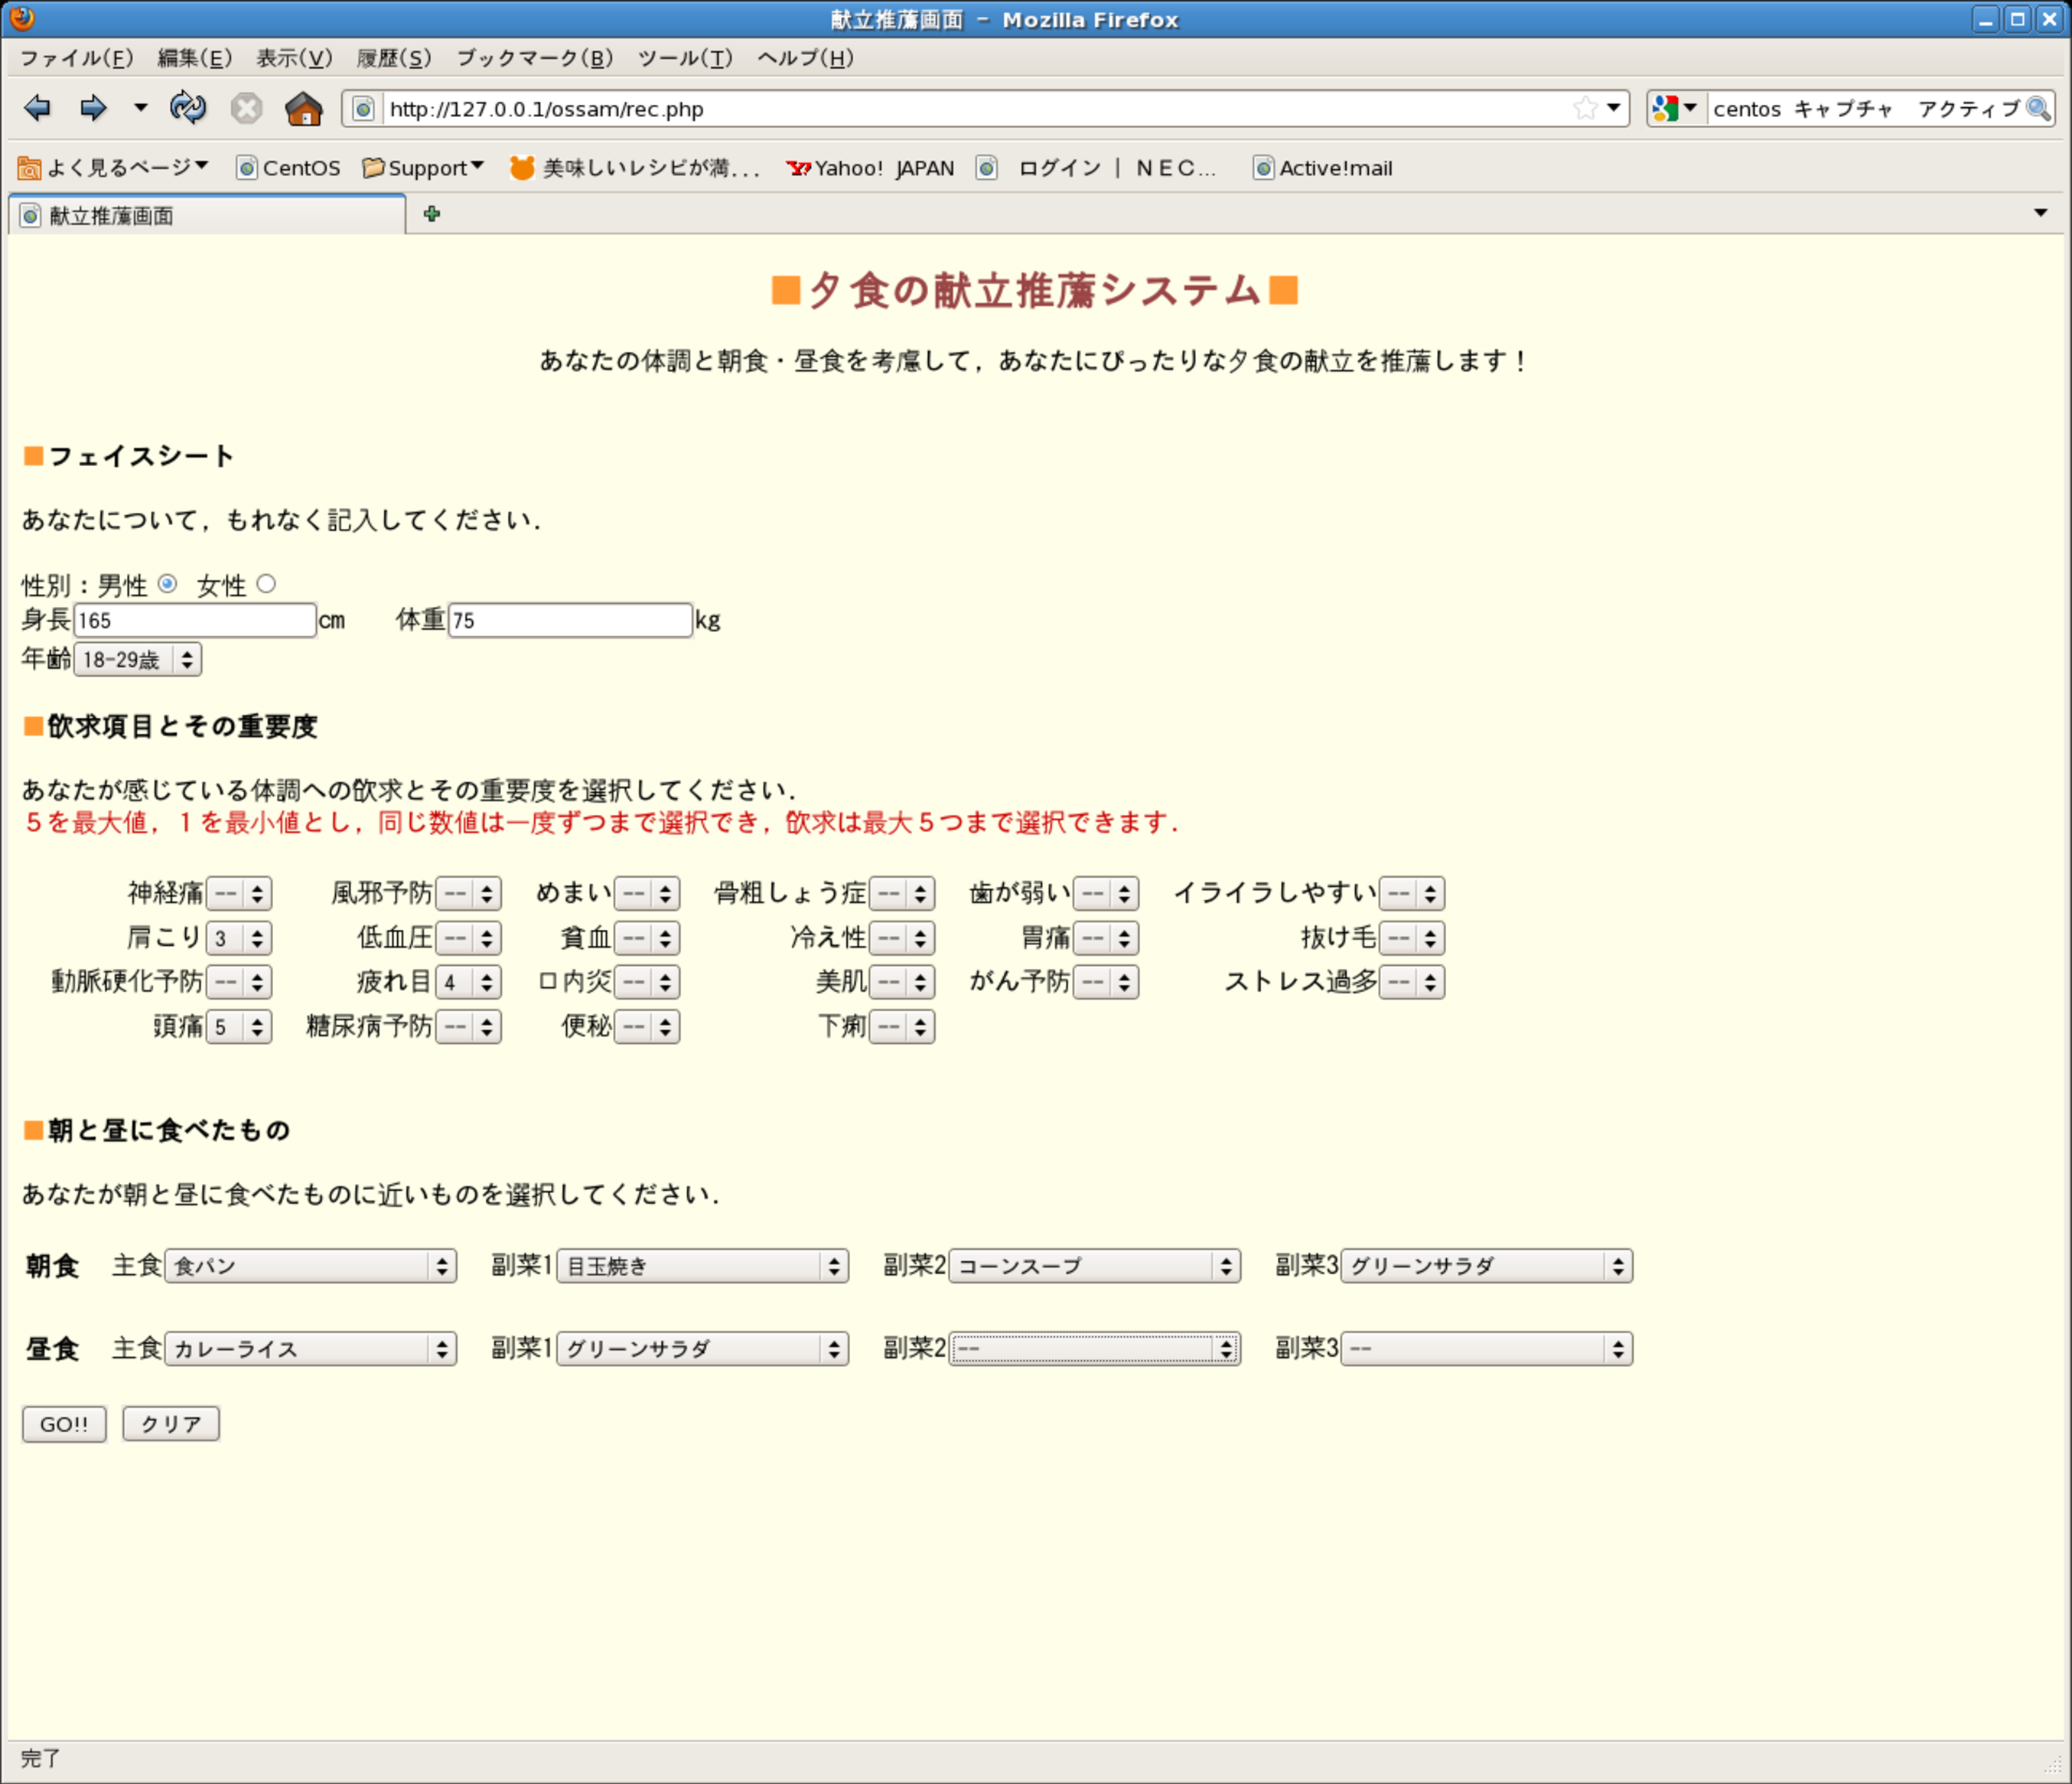
\includegraphics[scale=0.3]{input.eps}
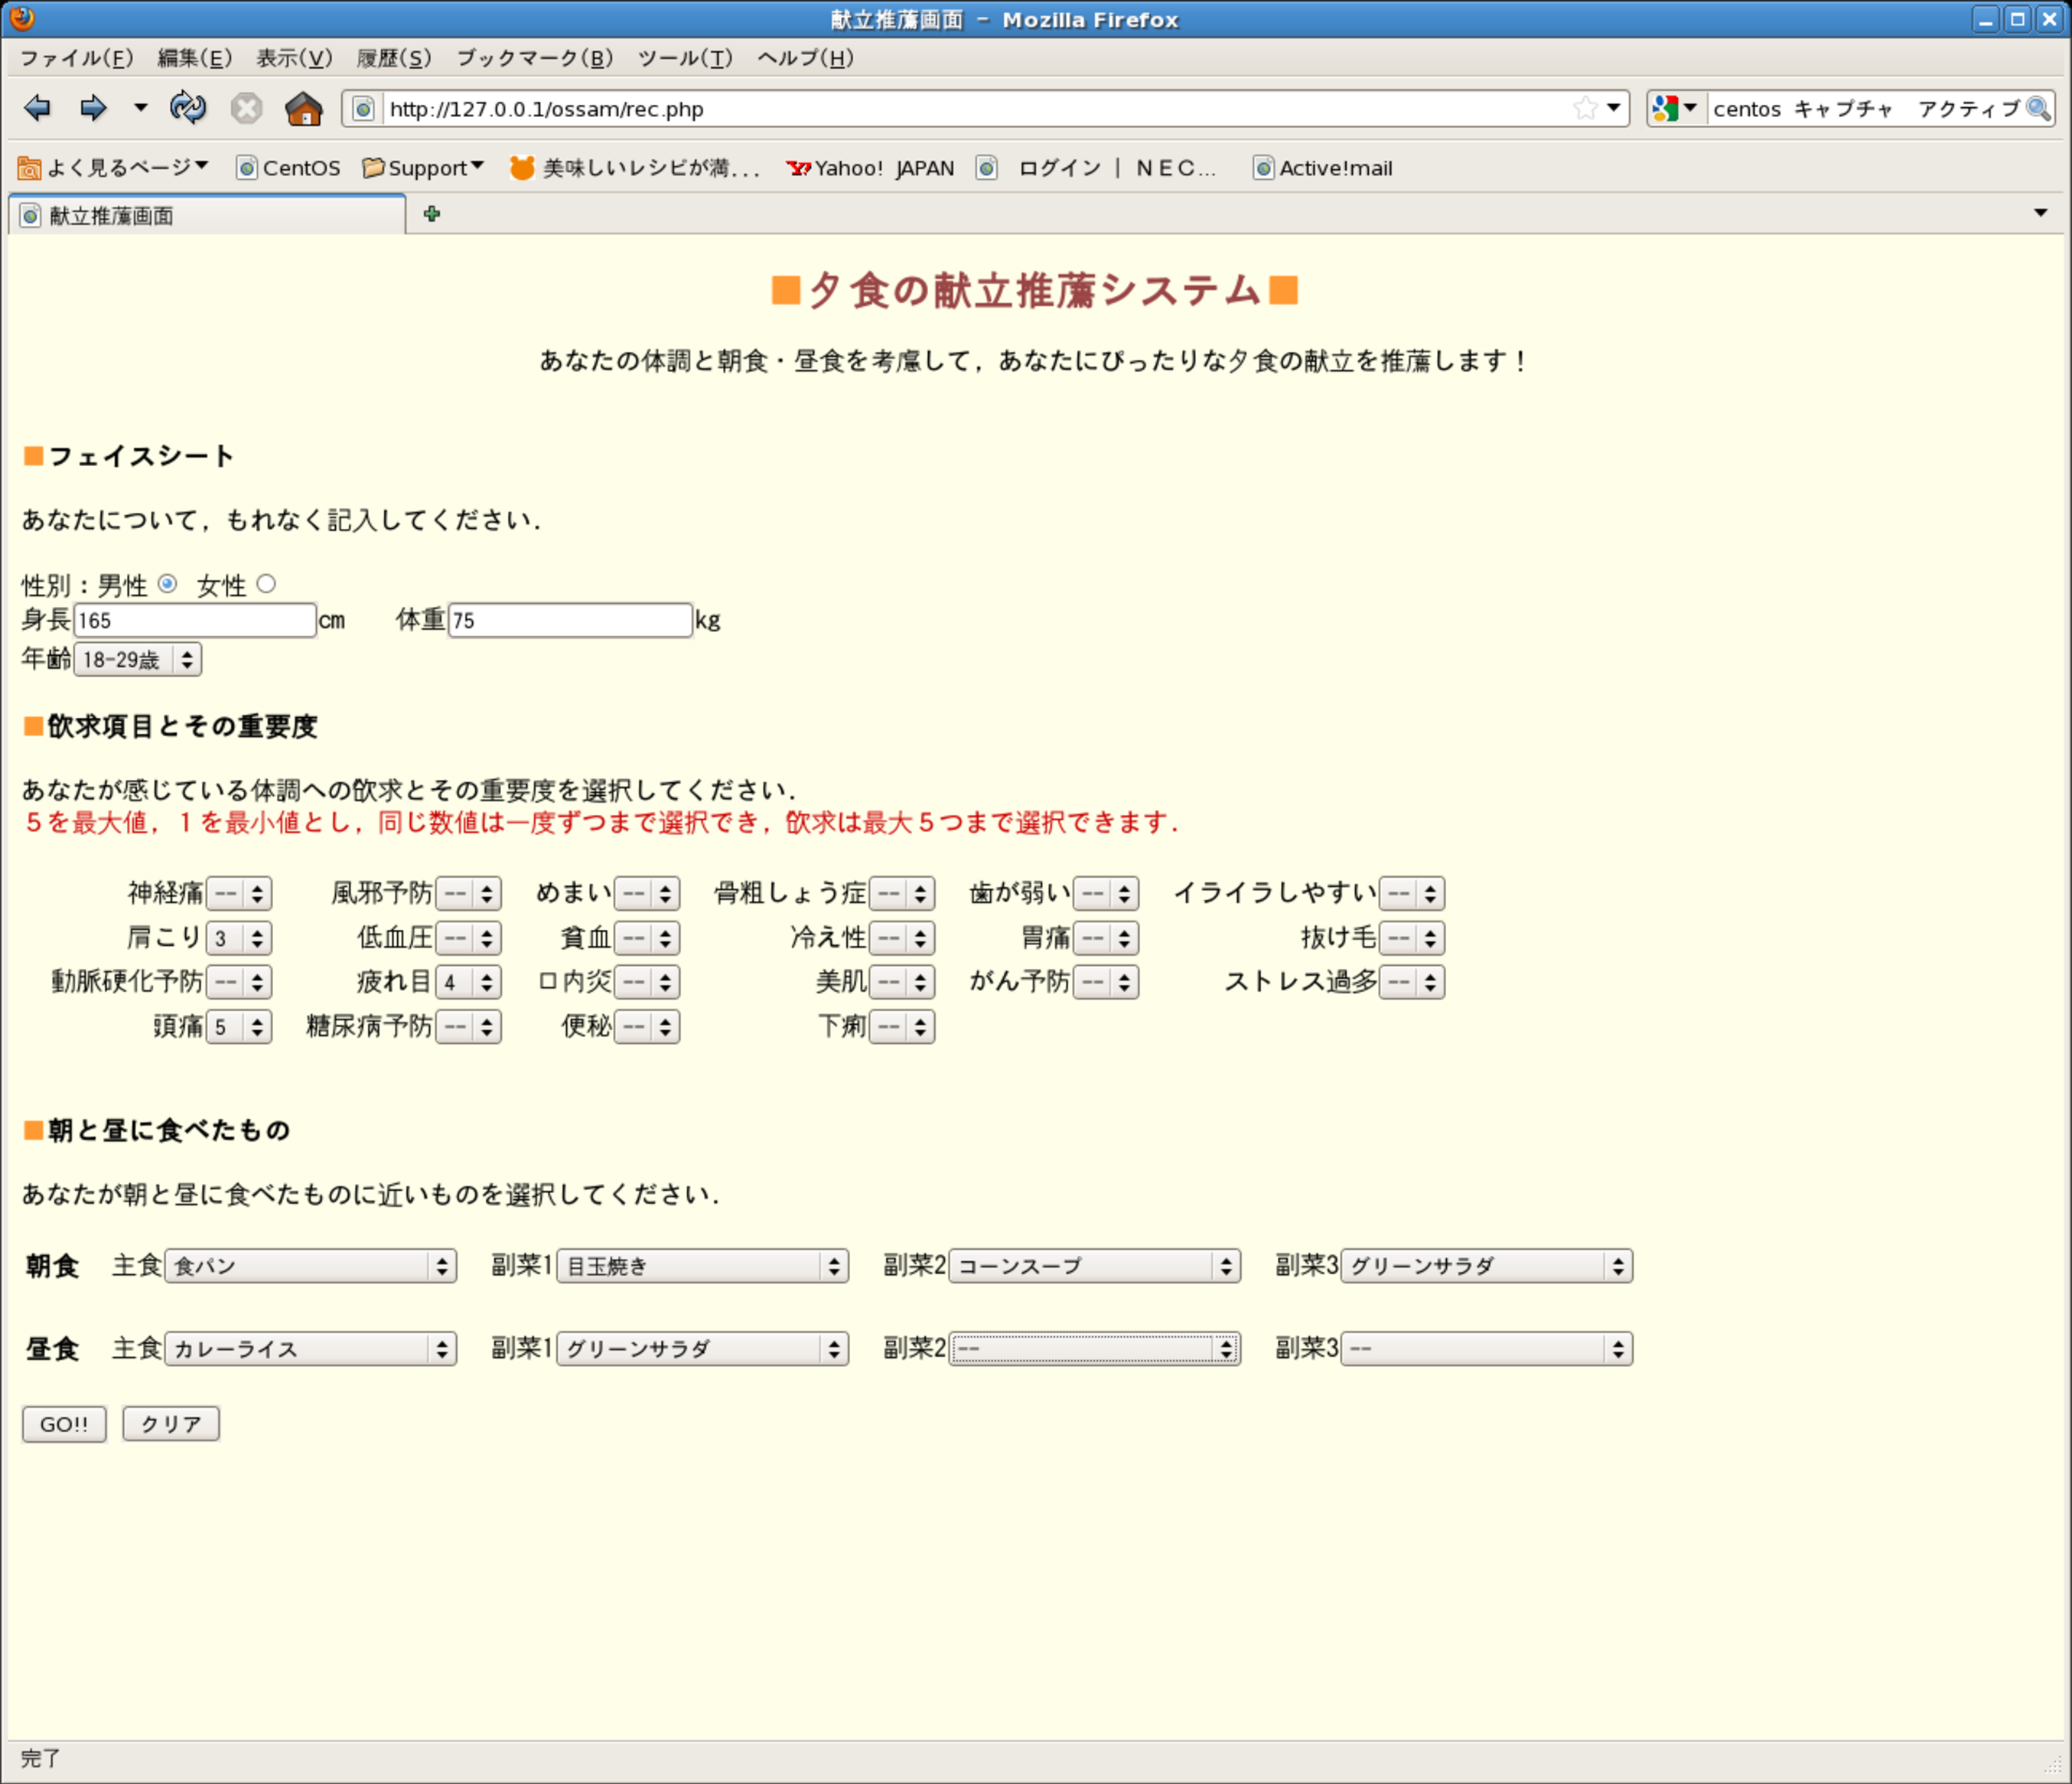
\includegraphics[scale=0.3]{input.pdf}
\caption{入力画面}
\label{fig:入力}
\end{figure}
\begin{table}[tbh]
  \caption{朝食,昼食での充足率}
  \label{tab:デモ1}
  \scriptsize
  \centering
    \begin{tabular}{c||cccccc}
      \hline
      不足順 & ビタミンD & ビタミンA & 食物繊維 & カルシウム & ビタミンB1 & カロリー\\
      \hline
      摂取割合(%) & 36 & 36.89 & 40.5 & 40.88 & 46.43 & 47.48\\
      \hline \hline
      不足順 & ビタミンE & 炭水化物 & ビタミンC & 亜鉛 & ビタミンB2 & 塩分 \\
      \hline
      摂取割合(%)& 50 & 55.22 & 58 & 58.44 & 58.75 & 65.4\\
      \hline \hline
      不足順 & 脂質 & 鉄分 & リン & 蛋白質 & コレステロール & \\
      \hline
      摂取割合(%)& 71.17 & 80.29 & 81.64 & 84.92 & 96.46 & \\
      \hline
    \end{tabular}
\end{table}


この表を踏まえて,充足率の計算から上位五品を主菜候補として提示する.
表示画面を図\ref{主菜}に示す.
\begin{figure}[tbh]
  \centering
% 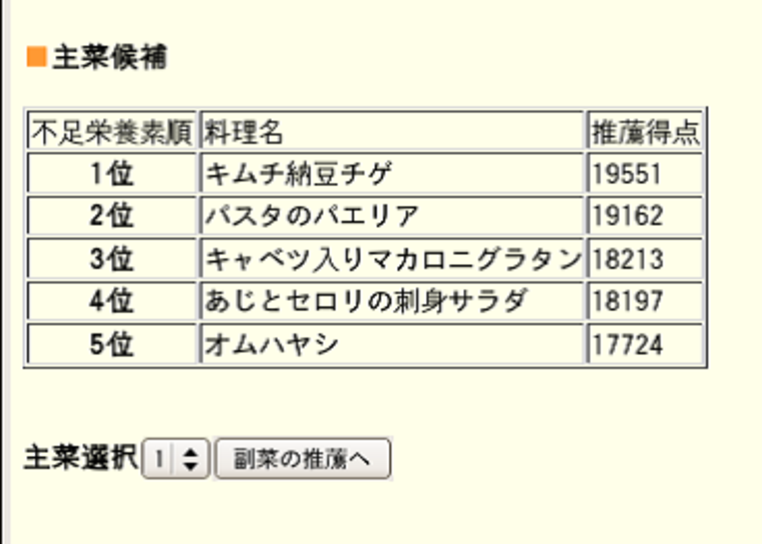
\includegraphics[scale=0.7,clip]{main3-2.eps}
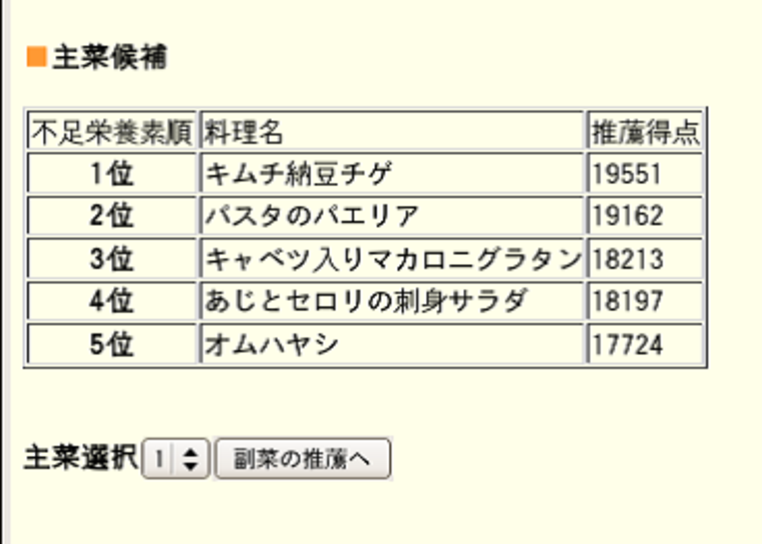
\includegraphics[scale=0.7]{main3-2.pdf}
\caption{主菜候補提示画面}
\label{主菜}
\end{figure}
\noindent
候補の中から主菜が選択された時,次の副菜1推薦画面\ref{副菜1}において選択されたレシピの写真と,
そのレシピに含まれる栄養素を摂取した場合の充足割合を表に表示し,副菜1の候補を上位五品提示する.
\begin{figure}[tbh]
  \centering
% 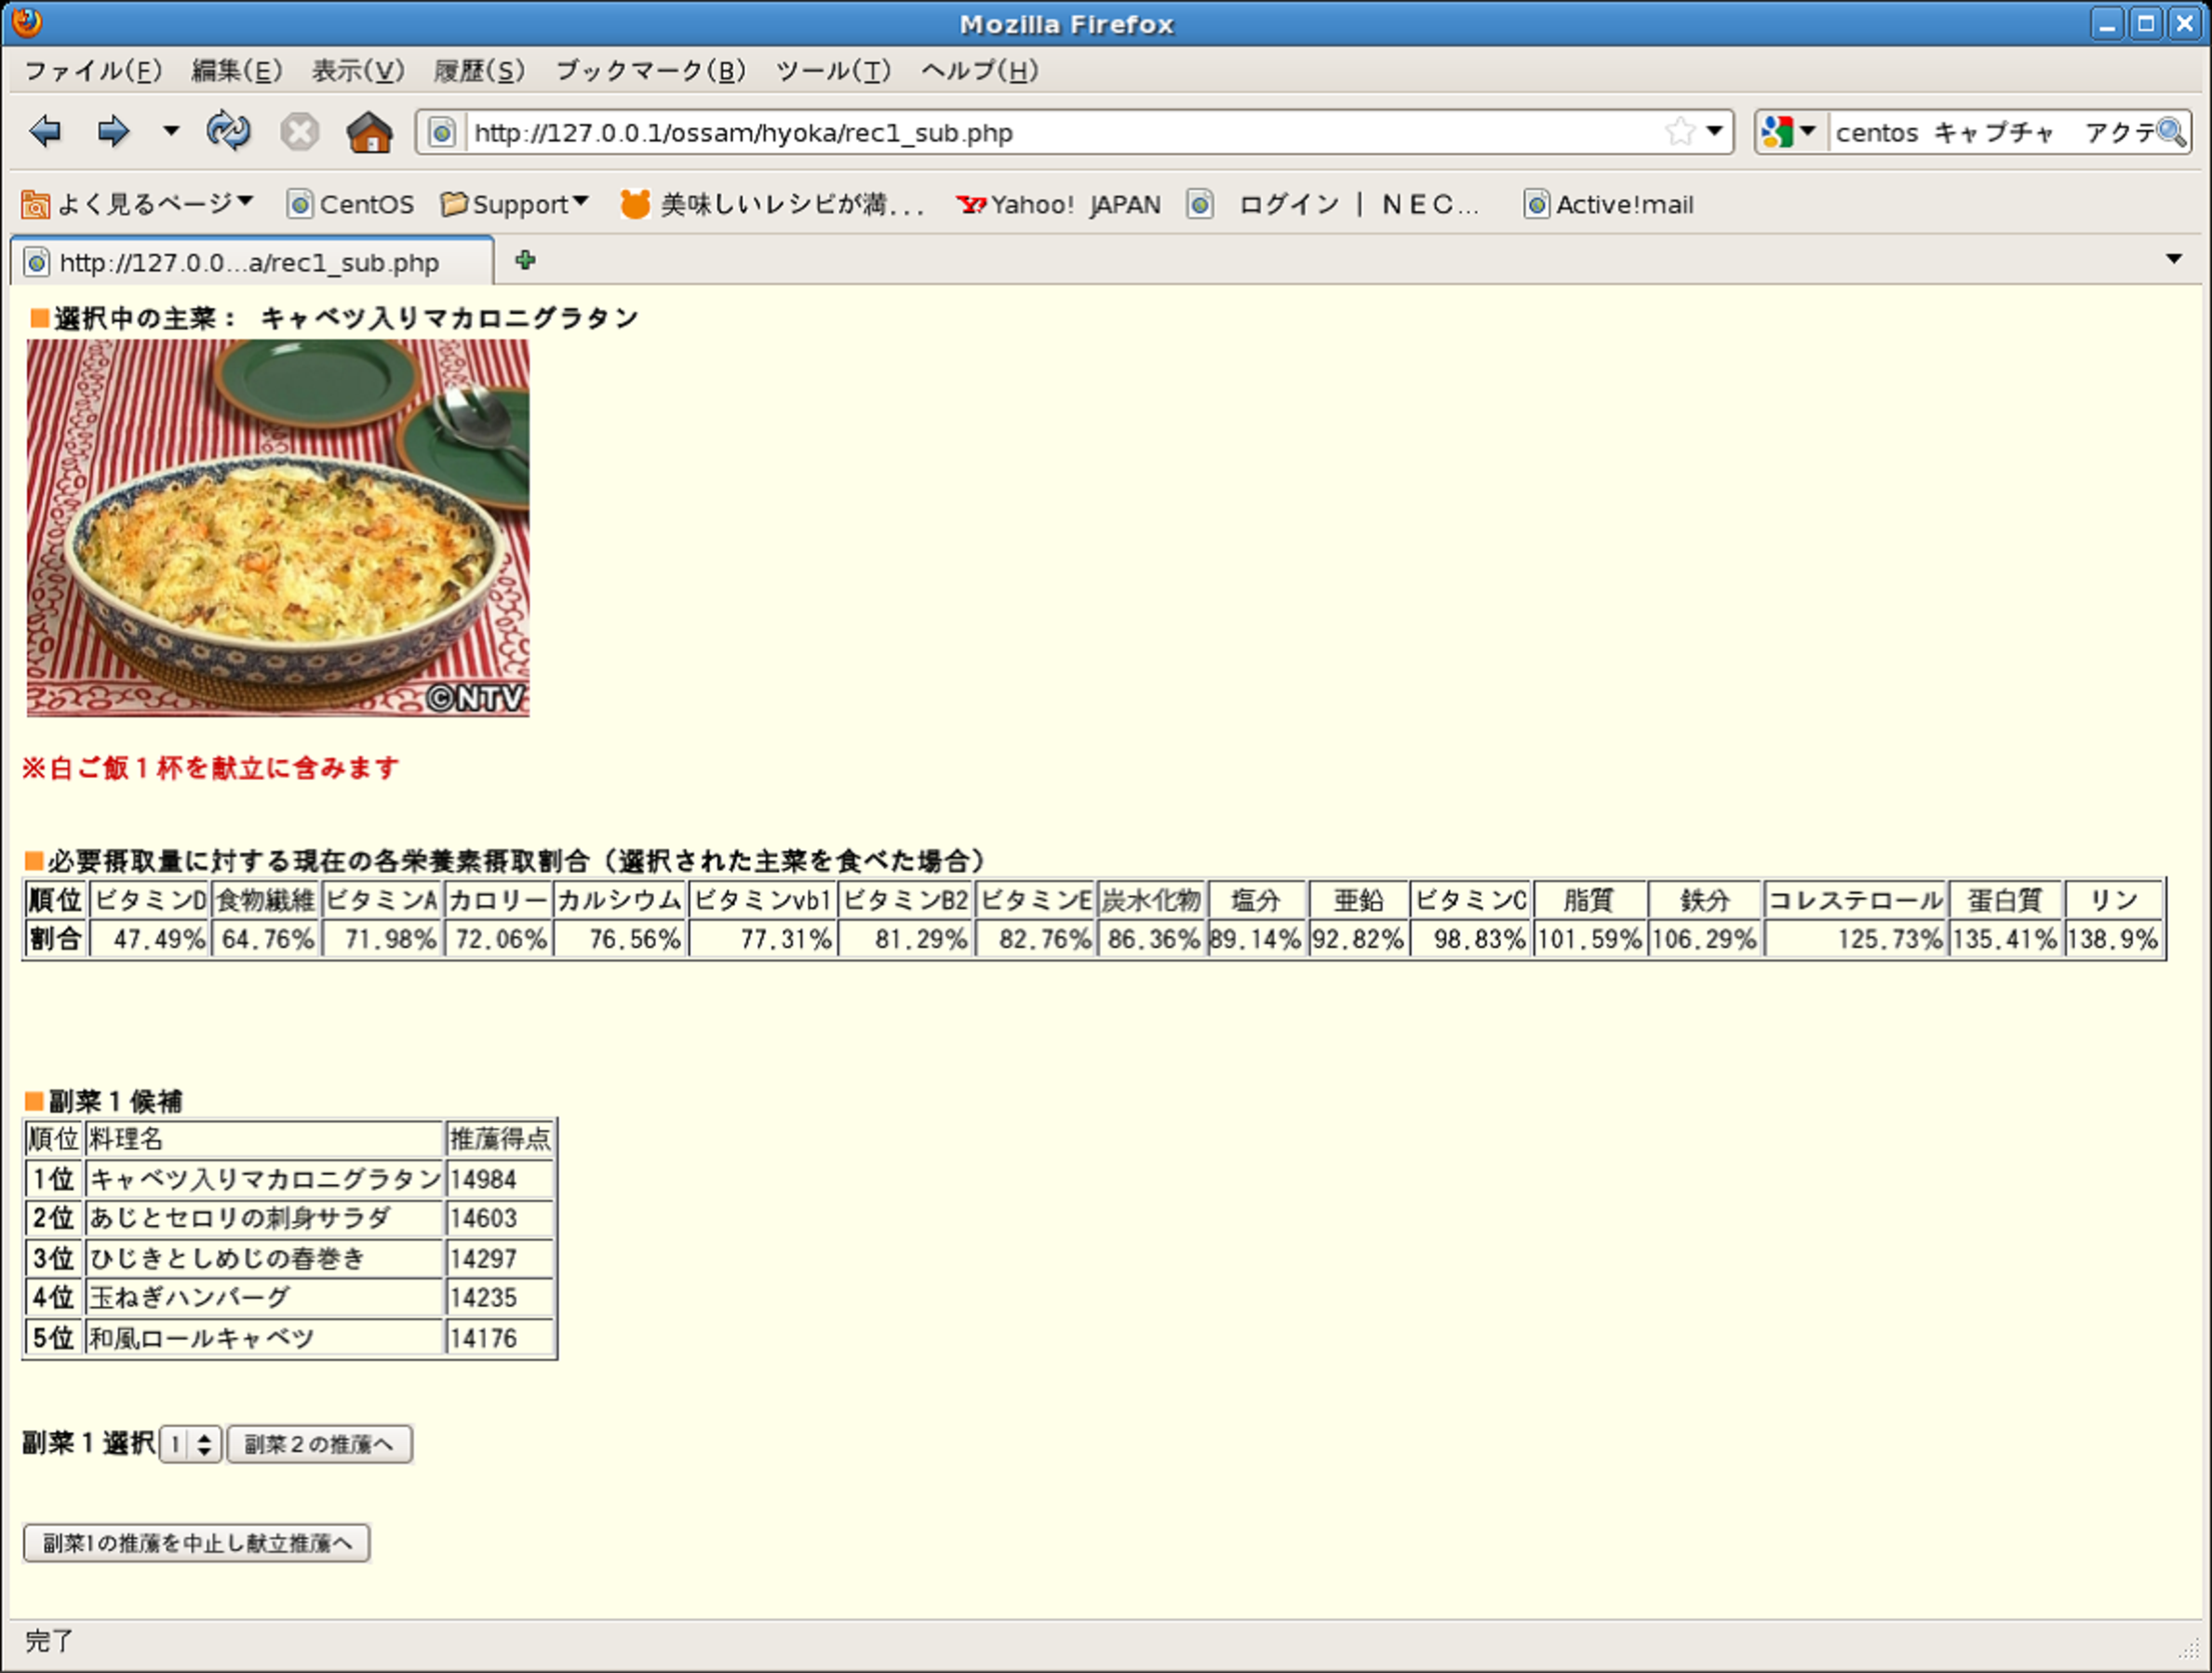
\includegraphics[scale=0.3,clip]{sub1-2.eps}
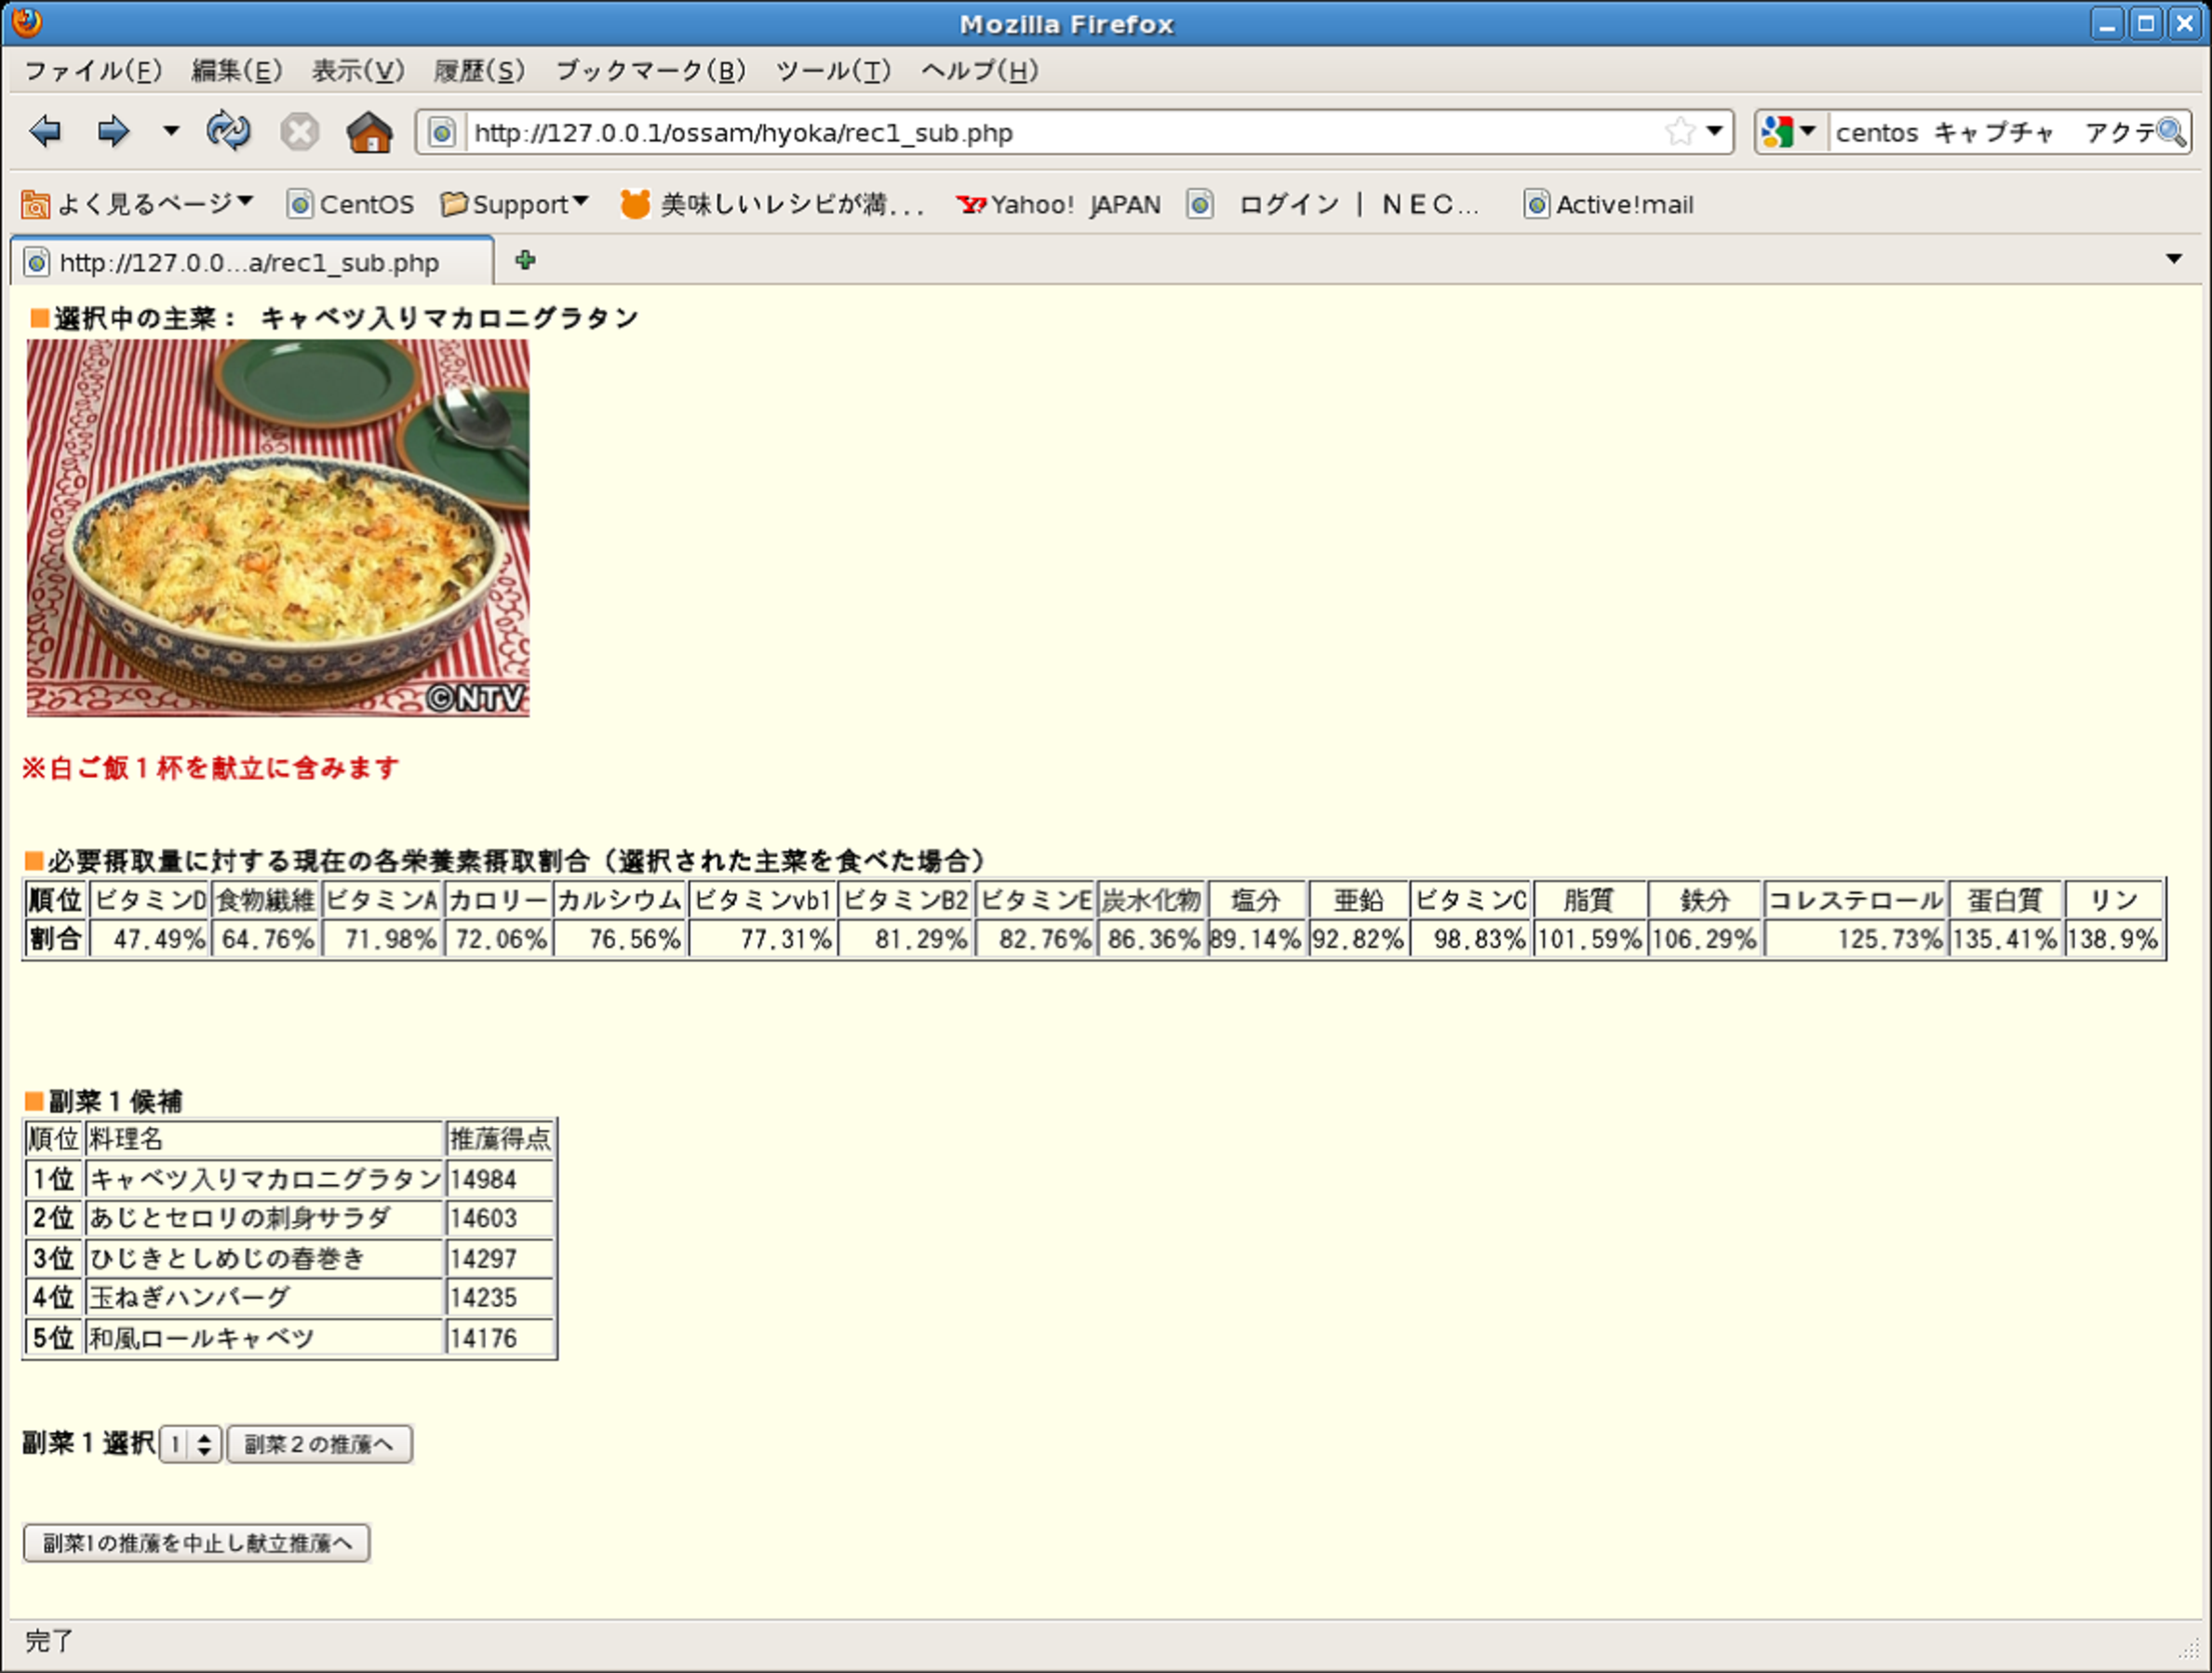
\includegraphics[scale=0.3]{sub1-2.pdf}
\caption{副菜1候補提示画面}
\label{副菜1}
\end{figure}
\noindent
この時,主菜で選択された料理が「キャベツ入りマカロニグラタン」であるため,
献立の中に白ご飯1杯分を含む.次に副菜の推薦を行うがこの時点で献立推薦を
終了したい場合のために「副菜の推薦を中止し献立推薦へ」というボタンを作成
した.
副菜1,副菜2と同様の処理を行い,最終的な献立推薦結果を図\ref{献立}に示す.


\begin{figure}[tbh]
  \centering
% 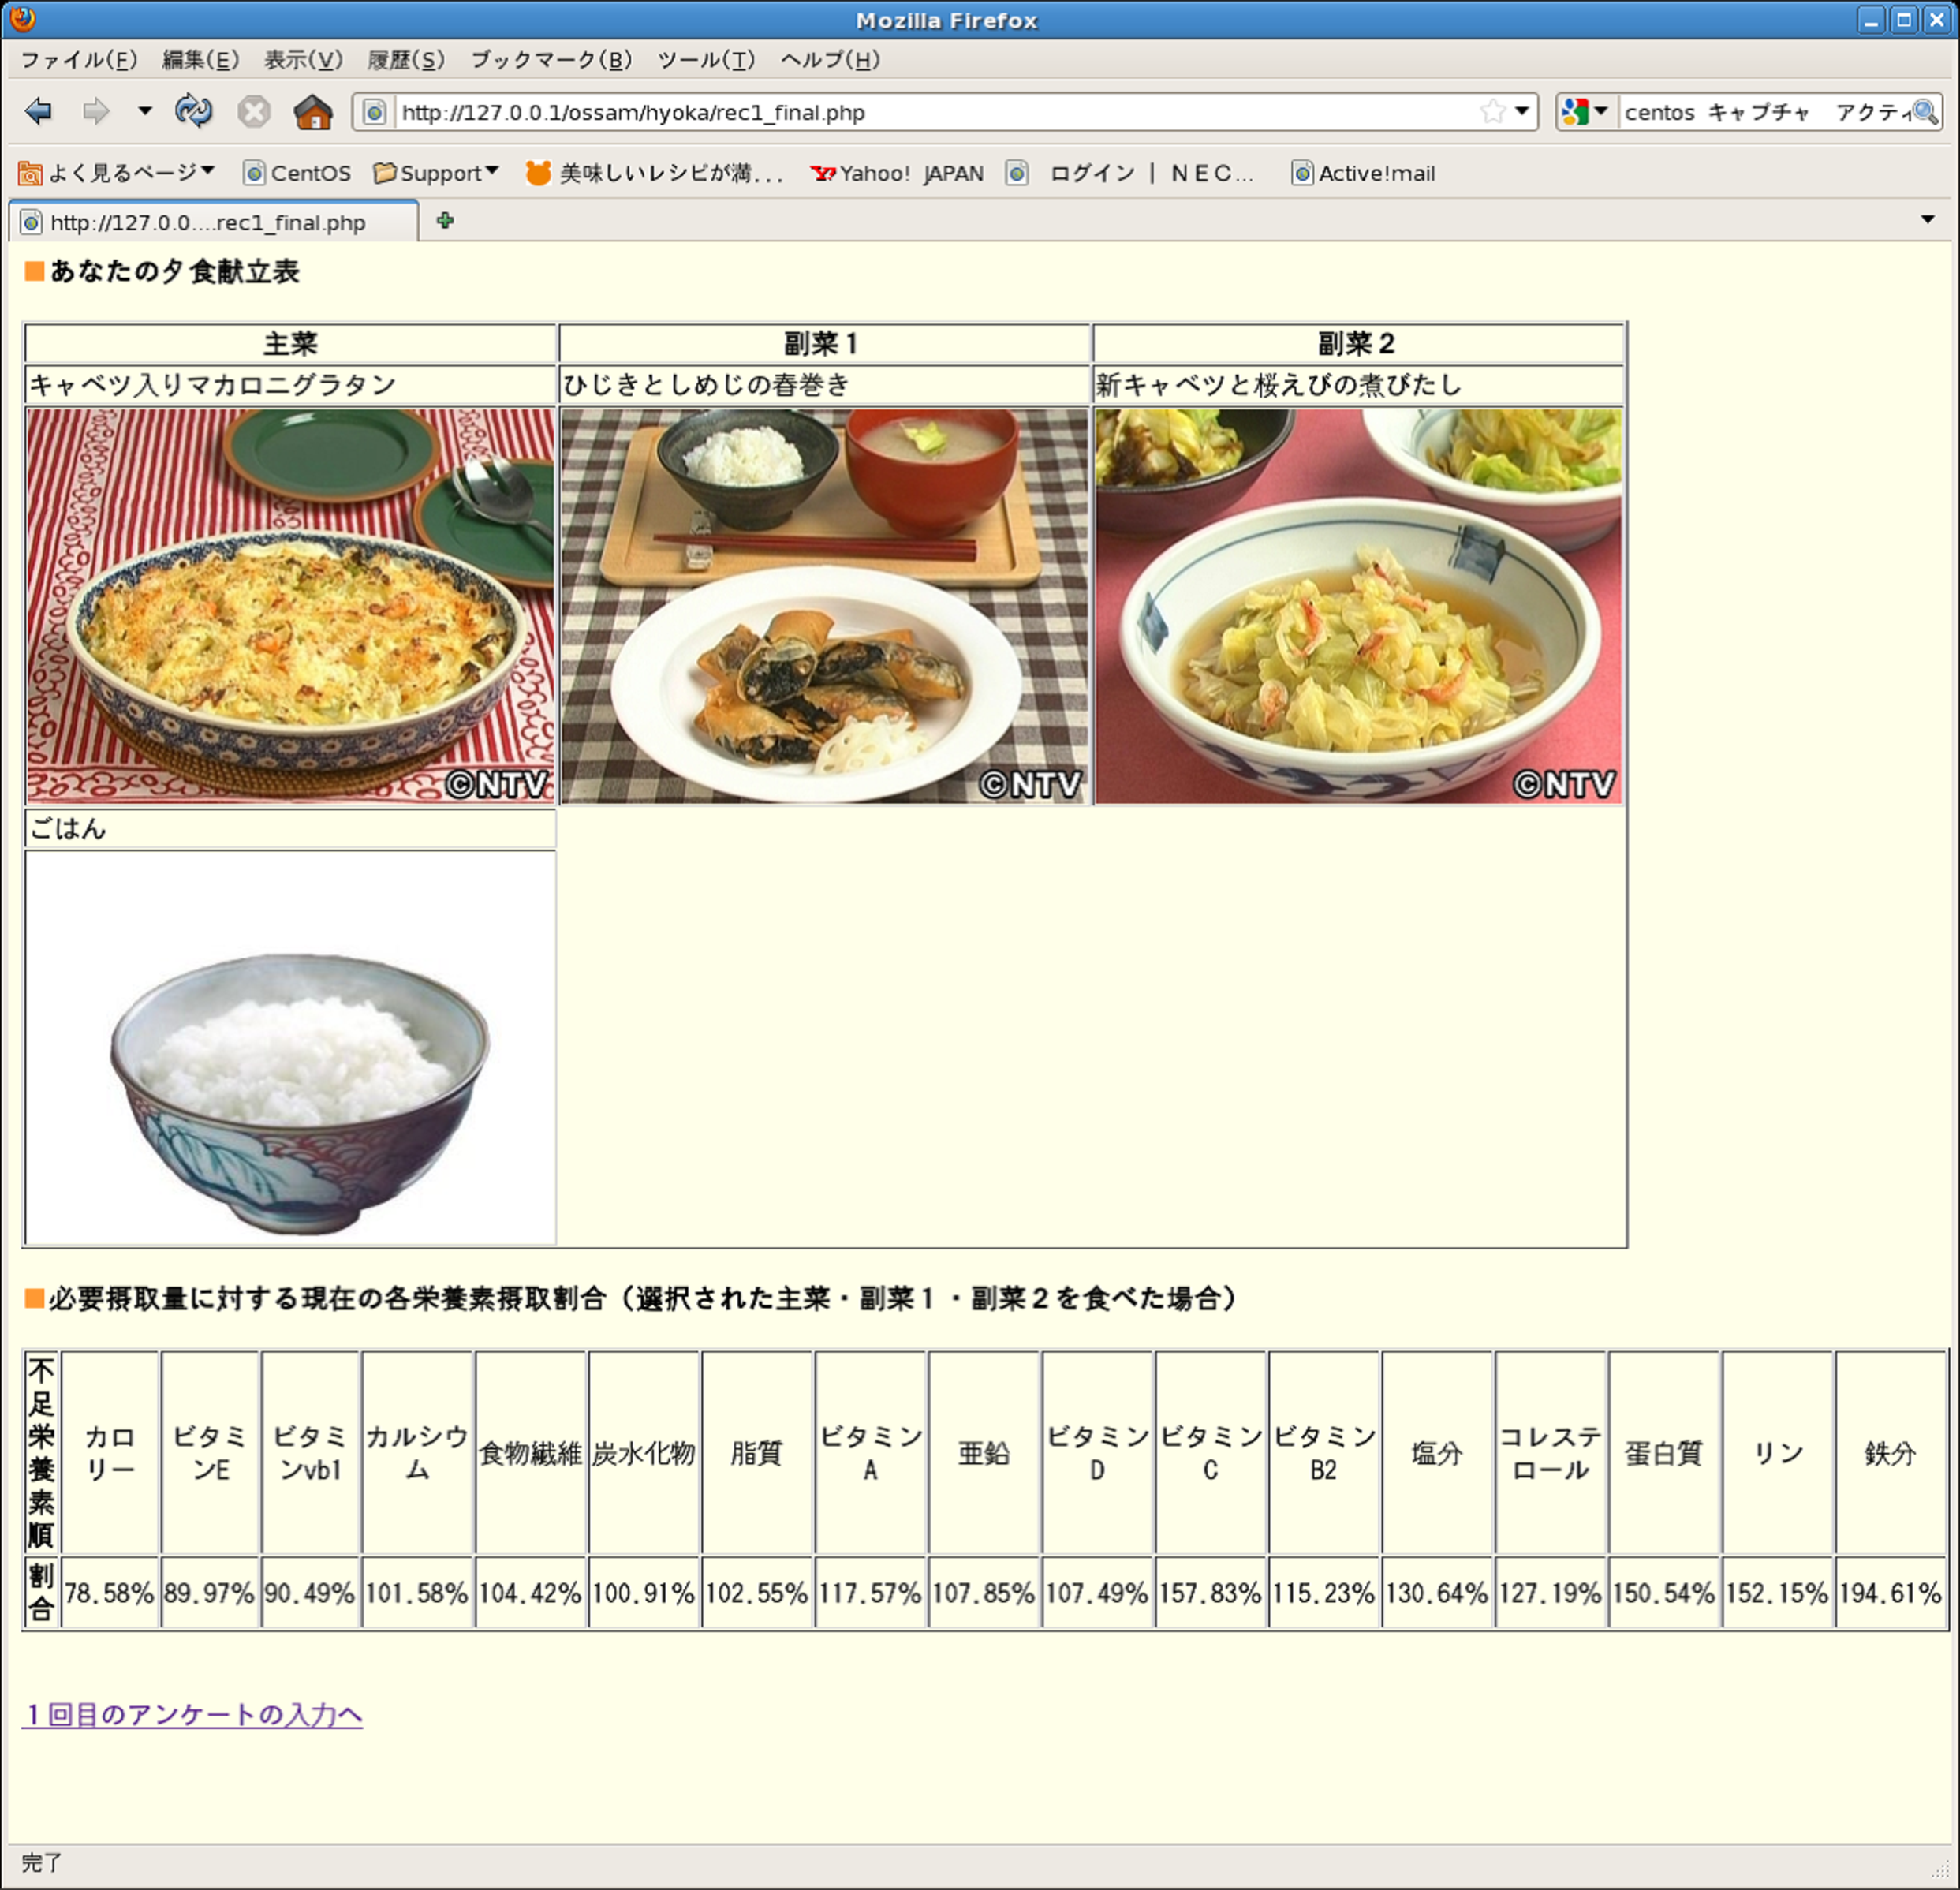
\includegraphics[scale=0.3,clip]{dinner.eps}
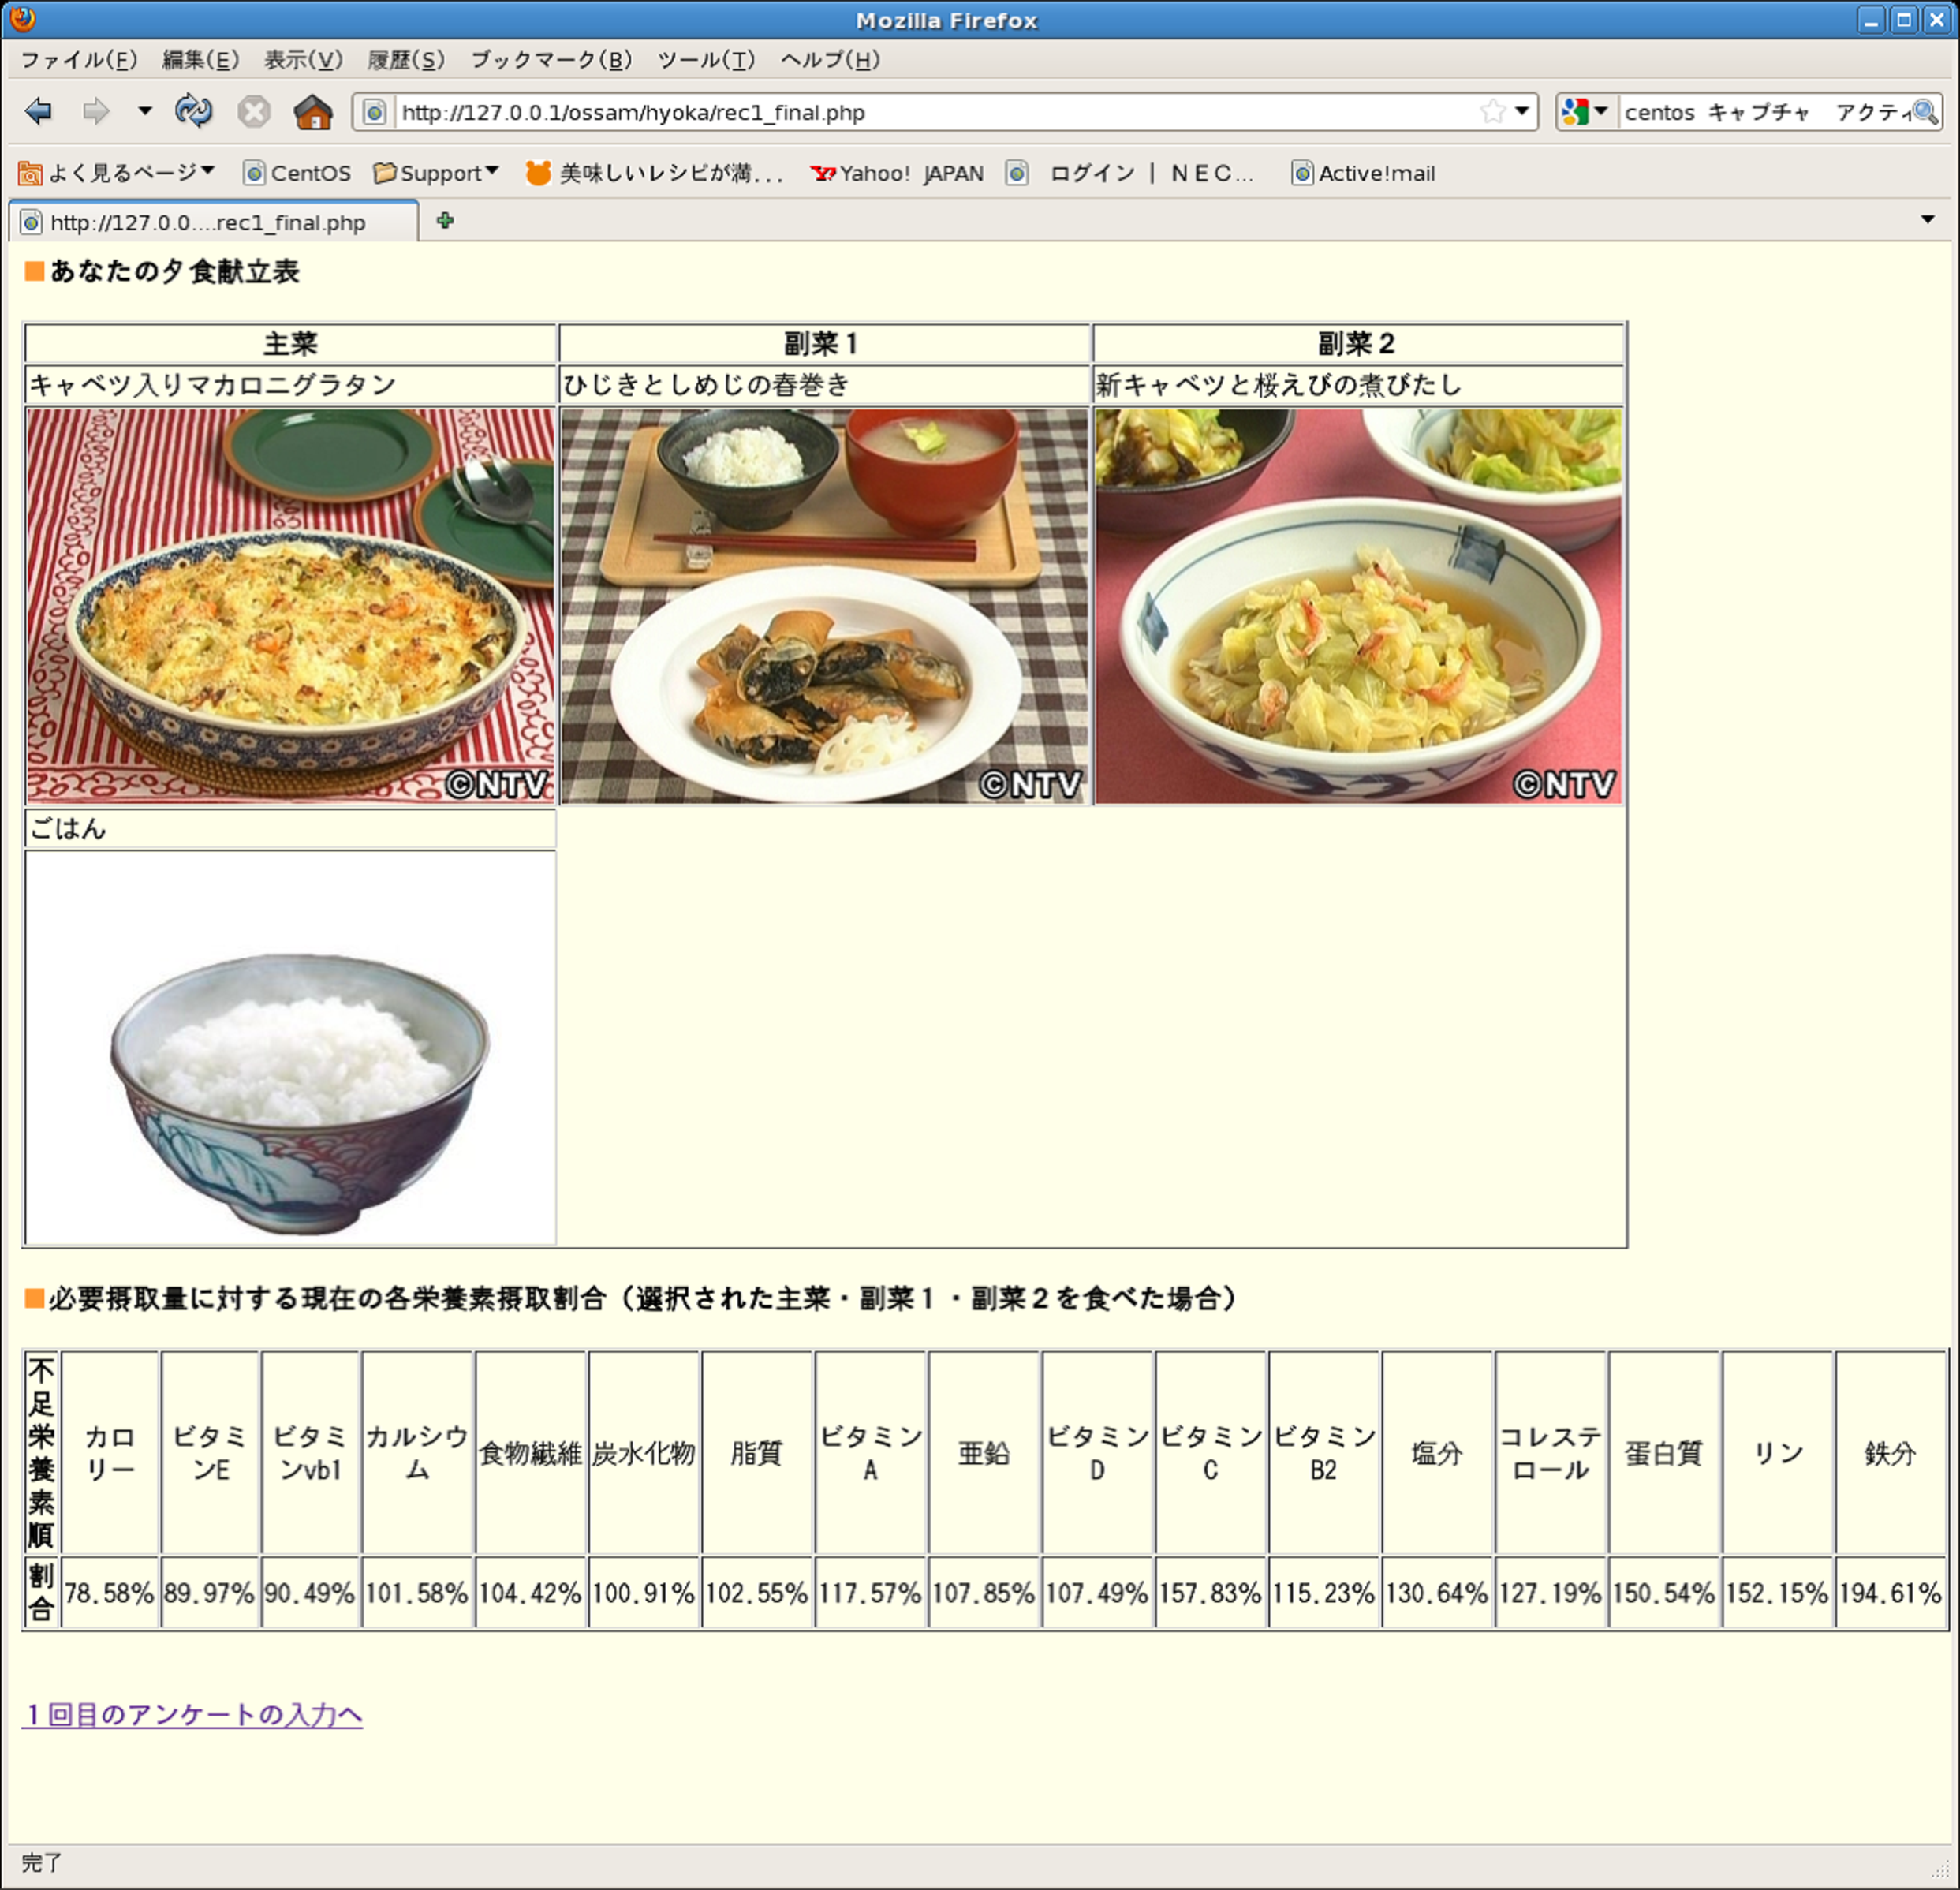
\includegraphics[scale=0.3]{dinner.pdf}
\caption{献立結果提示画面}
\label{献立}
\end{figure}

\chapter{評価実験}
第3章で述べた本研究の提案手法の有用性を検証するために,システムに対する
ユーザ評価を行った.
比較対象として栄養素バランスのみを考慮した献立推薦システムと,提案手法で
ある欲求項目を追加した献立推薦システムを構築し,それぞれに対する満足度を
男性14名,女性14名,計28名に対してアンケート調査を行い検証した.
アンケートの質問項目については表\ref{tab:アンケート}に示す.
\begin{table}[tbh]
  \caption{アンケート内容}
  \label{tab:アンケート}
  \centering
  \tiny
    \begin{tabular}{c|c|c}
      \hline
      質問番号 & 質問項目 & 回答項目\\
      \hline
      1 & 本システムを利用する際,各ページはわかりやすかったですか? & 5段階評価\\
      2 & フェイスシートでは十分満足のいく入力ができましたか? & 5段階評価\\
      3 & 推薦された料理で十分な栄養素バランスが摂取できたと感じますか? & 5段階評価\\
      4 & 推薦された料理を食べたくなりましたか? & 5段階評価\\
      5 & 献立を決める際に健康面の注意はしますか? & 5段階評価\\      
      6 & あなたの普段の食生活に一番近いものをお選びください. & 自炊,外食,お弁当・お惣菜,家族に作ってもらう \\
      7 & 本システムを利用し,気になった点があればご自由にご記入ください. & 自由記述 \\
      \hline
    \end{tabular}
\end{table}
\noindent
質問番号4を用いてユーザの満足度を調査した.これは「推薦システムを利用し
た際の納得感,満足感が高いからこそ推薦された献立を食べたいと感じる」とい
う概念により設定した.
回答を「非常に食べたいと思った」を5点,「まったく食べたいと思わなかった」
を1点として五段階に分けて集計を行った.
その結果,従来手法では平均4.036点,提案手法では平均4.464点となった.
この結果が有意に差があるといえるかどうかをt検定を用いて検証した.
t検定は二つのグループの平均の差が偶然誤差の範囲内にあるかどうかを調べる
ものである.
\begin{table}[tbh]
  \caption{t検定:一対の標本による平均の検定}
  \label{結果}
  \centering
    \begin{tabular}{ccc}
      \hline
        & 従来手法 & 提案手法\\
      \hline \hline
      平均 & 4.036 & 4.464\\
      分散 & 0.999 & 0.554\\
      観測数 & 28 & 28\\
      ピアソン相関 & 0.325 & \\
      仮説平均との差異 & 0 & \\
      自由度 & 27 & \\
      t & -2.194 & \\
      P(T\verb~<~=t)片側 & 0.019 & \\
      t境界値 片側 & 1.703 & \\
      P(T\verb~<~=t)両側 & 0.037 & \\
      t境界値 両側 & 2.052 & \\
      \hline
    \end{tabular}
\end{table}
\noindent
両側確率5%となる境界値を与えるtの値が式(4.1)を満たすとき,有意に差が
あるといえる.評価実験の結果を表\ref{結果}に示す.
\begin{equation}
|t値| > t境界値 両側
\end{equation}
t値は-2.5751となり,この絶対値はt境界値 両側の値,2.0518の絶対値を上回っ
たため,提案手法と従来手法は有意に差があるといえる.
よって従来手法よりも提案手法の方が有意にユーザ満足度が高いことが証明された.
本手法はユーザ満足度の観点から有用であることがいえる.

しかし,栄養素充足率の平均・分散を表\ref{充足率}を見ると,すべての栄養素
が目標量に近い状態で推薦されている推薦結果は少ないという問題が生じている
ことも判明した.
\begin{table}[tbh]
  \caption{栄養素充足率の平均と分散}
  \label{充足率}
  \centering
  \scalebox{0.85}{
    \tiny
    \begin{tabular}{cccccccccc}
      \hline
従来手法  &  energy  &  protein  &  lipid  &  carb  &  calcium  &  lynn  &  iron  &  zinc  &  va \\
平均  & 84.61214286 & 170.1860714 & 123.5467857 & 102.9267857 & 87.81 & 138.5467857 & 163.155 & 124.2192857 & 454.7196429 \\
分散  & 254.2951168 & 577.3790524 & 5941.816258 & 464.6158647 & 390.9919143 & 376.771529 & 1877.912804 & 642.2288852 & 106348.1294 \\
\hline
従来手法  &  vd  &  ve  &  vb1  &  vb2  &  vc  &  cholesterol  &  fiber  &  salt  &   \\
平均  & 95.4875 & 124.3475 & 111.6228571 & 97.98428571 & 136.9025 & 88.8875 & 99.88535714 & 118.7510714 &   \\
分散  & 7014.083004 & 1173.17824 & 479.0318776 & 491.6420602 & 1638.196119 & 2030.176897 & 429.9510892 & 804.2529739 &   \\
\hline \hline
提案手法  &  energy  &  protein  &  lipid  &  carb  &  calcium  &  lynn  &  iron  &  zinc  &  va \\
平均  & 84.21142857 & 162.9225 & 118.1760714 & 98.37107143 & 89.28428571 & 138.1153571 & 134.1414286 & 114.8925 & 402.5871429 \\
分散  & 306.125348 & 915.0072973 & 4867.951467 & 500.8257096 & 813.1191316 & 967.5110034 & 1981.283905 & 857.2042616 & 71441.99344 \\
\hline
提案手法  &  vd  &  ve  &  vb1  &  vb2  &  vc  &  cholesterol  &  fiber  &  salt &    \\
平均  & 105.5932143 & 95.29678571 & 105.9567857 & 87.38071429 & 117.5817857 & 85.86071429 & 100.6325 & 120.54 &    \\
分散  & 7051.922665 & 448.5906432 & 901.1016218 & 624.1289566 & 1074.719072 & 2681.537299 & 522.3062402 & 1035.743786 &    \\
      \hline
    \end{tabular}
}
\end{table}
\noindent
これは,献立推薦を行う差異にユーザ自身で主菜,副菜の候補から料理を選択で
き,さらに途中で副菜の推薦を中断できるようにしたため,充足率を満たす前に
推薦が終了されてしまったことが原因と考えられる.

\chapter{おわりに}
本研究では,従来の栄養素バランスを考慮した推薦に加え,さらにユーザの体調
や欲求を反映させた献立推薦の手法を提案した.
具体的には,ユーザの状況を把握するための欲求項目の設置を行った.
これにより,ユーザの欲求や体調を自動的に献立推薦へ反映させることが可能となる.
また評価実験により,この状況を把握した上での栄養素バランスを考慮した提案
手法を用いたシステムは従来の栄養素バランスのみを考慮した献立推薦に比べて
優位にユーザ満足度が高いことが示された.

今後,栄養素充足率をすべての栄養素に対して目標量に過不足なく推薦するために,
候補とするレシピデータ数の増加や,推薦アルゴリズム中の栄養素充足率に関す
る制約の修正を行っていく.

%%
%% 謝辞
%%
\acknowledgements
\addcontentsline{toc}{chapter}{謝辞}

本論文を作成するにあたり,多大なるご指導を賜りました新島 襄 教授,
新島 八重 教授,ドウェイト・ウィットニー・ラーネッド 教授,
ジェローム・デイヴィス 教授に厚く御礼申し上げる.
最後に,卒業に至るまでの間ご指導いただいた諸先生方ならびに研究室
メンバの皆様に心からの感謝の意を表す.
\newpage

%%
%% 参考文献
%%
\makeatletter
\renewenvironment{thebibliography}[1]
{\chapter*{\bibname\@mkboth{\bibname}{\bibname}}%
 \addcontentsline{toc}{chapter}{\bibname}% この行追加
   \list{\@biblabel{\@arabic\c@enumiv}}%
        {\settowidth\labelwidth{\@biblabel{#1}}%
         \leftmargin\labelwidth
         \advance\leftmargin\labelsep
         \@openbib@code
         \usecounter{enumiv}%
         \let\p@enumiv\@empty
         \renewcommand\theenumiv{\@arabic\c@enumiv}}%
   \sloppy
   \clubpenalty4000
   \@clubpenalty\clubpenalty
   \widowpenalty4000%
   \sfcode`\.\@m}
  {\def\@noitemerr
    {\@latex@warning{Empty `thebibliography' environment}}%
   \endlist}
\makeatother
\bibliographystyle{jplain}
%\nocite{*}
\bibliography{publication}

%%
%% 付録
%%
\appendix
\chapter{表紙,中表紙,要旨・概要,目次}
\setcounter{page}{1}
\renewcommand{\thepage}{\thechapter-\arabic{page}}
「同志社大学文化情報学部卒業論文/大学院文化情報学研究科修士・博士論文用
スタイルファイル」 (以下学位論文スタイルファイルと呼ぶ) では,卒業論文,
修士・博士論文専用の表紙,中表紙,要旨・概要ページ,目次ページ,本文,付
録を出力する\footnote{卒業論文,修士論文,博士論文を提出する際は,別のス
タイルファイルが用意されている概要ページ (卒業論文)・紀要「文化情報学」
掲載用概要 (修士・博士論文),論文本体 (表紙,中表紙,要旨・概要ページ,
目次ページ,本文,そして付録を片側印刷して作成する冊子体) の二種類が必要
である.}.

表紙,中表紙,要旨・概要,目次ページの作成に必要な項目は,
\begin{itemize}
  \item 論文のタイトル,要旨・概要の内容
  \item 論文の著者名
  \item 主担当,副担当教員名 (卒業論文のみ)
  \item 卒業論文/修士論文/博士論文の設定
  \item 学科名/課程
  \item 学籍番号
  \item 入学年度,卒業年度
  \item 提出日 (卒業論文のみ)
\end{itemize}
である.なお,印刷後に中表紙の学籍番号の下に手書きで氏名を記述する.
これらのデータは,\verb|\makecover| によって 1 ページ目をシール用紙に印
刷してバインダーの表紙に貼るためのタイトルページが出力されるほか,
\verb|\makeicover| によって中表紙ページが 2 ページ目に,
\verb|\abstractpage| によって要旨・概要ページが 3 ページ目に,
\verb|\tableofcontents| によって目次ページが 4 ページ目以降に出力される
.

このサンプルソースでは,目次だけを出力しているが,別に図目次
(\verb|\listoffigures|) や表目次 (\verb|\listoftables|) を出力することも
できる.出力の必要がある場合は,それぞれのコマンドのコメントアウトを外せ
ばよい.

\section{論文のタイトル,要旨・概要}

\subsection{title}
論文のタイトルを記述する.タイトルが長い場合は途中で \verb/\\/ コマンド
を入れ,おかしな部分で改行されないように工夫する.
本学位論文スタイルファイルでは日本語タイトルだけを定義しているが,将来的
には英文タイトルも出力できるよう仕様変更する予定である.

\subsection{abstract}
論文の要旨・概要に記述するテキストを記述する.
また,タイトル同様,本学位論文スタイルファイルでは日本語の要旨・概要だけ
を定義しているが,将来的には英文要旨も出力できるよう仕様変更する予定であ
る.

\section{論文の著者名,主担当・副担当教員名,論文の種類}
\subsection{author}
論文の著者名を記述する.姓と名の間に半角スペースを必ず入れること.

\subsection{advisers (卒業論文のみ)}
論文の主担当教員名,副担当教員名を記述する.
姓と名,名と称号の間に半角スペースを必ず入れること.
現在の論文スタイルファイルの仕様では最大四名までの主担当教員,副担当教員
を記述することができるが,四名以下の場合は,単に該当行を削除するのではな
く,例に挙がっているように \verb|{}{}| を利用すること.

\subsection{bachelor/master/doctor}
論文の種類を指定する.
卒業論文の場合には \verb|\bachelor| を,
修士論文の場合には \verb|\master| を,
また博士論文の場合は \verb|\doctor| を設定する.

\section{所属学科・課程,学籍番号,入学年度,卒業/修了年度,論文提出日}

\subsection{department}
学部の場合は所属学科,大学院の場合は課程を記述する.
記述内容には三種類あるが,該当以外はコメントアウトしておく.

\subsection{studentid}
学籍番号を記述する.

\subsection{eyear,gyear}
\verb|\eyear| に入学年度を,\verb|\gyear| に卒業/修了年度を記述する.
例えば,2010 年 3 月に卒業/修了する者の卒業/修了年度は 2009 となる.

\subsection{date (卒業論文のみ)}
論文提出日を記述する.

\section{研究業績 (修士・博士論文のみ)}

修士・博士論文に関する研究業績を記述する.
業績の列挙には,{\tt thebibliography} 環境などを用いる.

\section{製本}

\subsection{バインダ}
印刷した論文はバインダに綴じて提出する.バインダは生協購買部で販売してい
る「CE-4K (紙製)」を使用する.
シールは,生協購買部で販売している「コピー \& レーザー \& インクジェット
用 タックシール IJR-A4N 上質粘着紙 10 Sheets」を用いる.
表紙は,論文の 1 枚目に作成されるものをシールに印刷し,バインダに貼付す
る.
背表紙は同梱の {{\tt splines.tex}} を用い印刷する.
なお,このファイルは A4 一枚で三人分印刷可能なので,研究室内で適宜調整し,
シールを無駄にしないようにする.

\subsection{製本}
提出するものは,概要 1 枚と論文本体 3 部である.
バインダに綴じる論文本体は以下の構成にする.なお,2 枚目に作成される中
表紙の学籍番号の下に,氏名を手書きで記入すること.
\begin{enumerate}
  \item 白紙
  \item 中表紙
  \item トレーシングペーパー (修士・博士論文のみ)
  \item 提出者の写真 (修士・博士論文のみ)
  \item 要旨・概要
  \item 目次
  \item 本文
  \item 参考文献
  \item 付録
  \item 特記事項 (修士・博士論文のみ)
  \item 白紙
\end{enumerate}

%%
%% 特記事項 (修士・博士論文のみ.卒業論文の場合はコメントアウトすること)
%%
%\newpage
%\chapter{特記事項}
%\section*{研究論文}
%\thispagestyle{empty}
%\begin{enumerate}
%	\item 同志社太郎. ○○○○の提案. 文化情報学, Vol. X, No. X, 
%		pp. 1--8, June 20XX.
%	\item 同志社太郎. ××××の提案. 文化情報学, Vol. XX, No. XX, 
%		pp. 12--19, April 20XX.
%\end{enumerate}
%
%\section*{受賞}
%\begin{enumerate}
%	\item ○○学会 第○回全国大会 学生奨励賞, June 20XX.
%\end{enumerate}
%
%\section*{著書}
%\begin{enumerate}
%	\item 同志社太郎. データベースシステム. ○○出版, May 20XX.
%\end{enumerate}
%
%\section*{社会活動}
%\begin{enumerate}
%	\item ○○学会 第○回○○研究会 ローカル担当, June 20XX.
%\end{enumerate}
%
%\section*{研究又は教育に係る補助業務}
%\begin{enumerate}
%	\item データベースシステム,ティーチング・アシスタント,20XX.
%	\item 情報アクセス技術,ティーチング・アシスタント,20XX.
%\end{enumerate}

\chapter{バージョン履歴}
\begin{itemize}
  \item 2008/4/20: 初版作成
  \item 2009/1/12: 第二版作成
  \item 2009/11/12: 第三版作成
  \item 2010/10/5: 第四版作成
  \item 2010/11/30: 第五版作成
  \item 2011/12/1: 第六版作成
  \item 2013/12/1: 第七版作成
  \item 2013/12/12: 第八版作成
  \item 2017/6/8: 第九版作成
\end{itemize}


\end{document}
